\documentclass[oribibl,envcountsame,dvipdfmx]{llncs}
\usepackage{adjustbox}
\usepackage[linesnumbered,ruled,vlined]{algorithm2e}
\usepackage{algorithms/algorithmic}
\usepackage{booktabs}
\usepackage{amsmath}
\usepackage{amssymb}
%\usepackage{bmpsize} %%% senda
%\usepackage{amsthm}
\usepackage{booktabs}
\usepackage[shortlabels]{enumitem}
%\usepackage{forest}
\usepackage{latexsym}
\usepackage{mathrsfs}
%\usepackage{multirow}
%\usepackage{pgfplots}
%\usepackage{pgfplotstable}
%\usepackage{thmtools}
\usepackage{xspace}
\usepackage{here}

\setlist[itemize]{itemsep=1pt}
%\SetAlgorithmName{Algorithm}
%\usetikzlibrary{patterns,arrows,decorations,shapes}
%\tikzset{
%	transv/.style={-latex,thick,rounded corners=12pt,shorten >=5pt,shorten <=5pt},
%	transh/.style={transv,densely dotted},
%	ID/.style={label={[anchor=south east,inner sep=2pt]north east:#1}},
%}
%\forestset{
%	Node/.style={draw,circle,fill=black,minimum width=12pt,inner sep=0},
%	Subtree/.style={triangle,draw=none,fill=none,minimum width=40pt,inner sep=0},
%	Leaf/.style={rectangle split,rectangle split parts=2,minimum height=100pt,ID=#1,draw,inner sep=1pt},
%	Inter/.style={circle,ID=#1,outer sep=5pt,draw,inner sep=1pt},
%	Leafn/.style={ID=#1,draw,inner sep=1pt,minimum width=14pt,minimum height=14pt},
%	Intern/.style={circle,ID=#1,draw,inner sep=1pt,minimum width=14pt,minimum height=14pt},
%}
%\renewcommand{\baselinestretch}{0.98}
%\topmargin=-1.0cm
%\oddsidemargin=0.4cm
%\evensidemargin=0.4cm
%\textheight=20.0cm
%\textwidth=15.0cm

\sloppy

%\_\_\_\_\_\_\_\_\_\_\_\_\_\_\_\_
% macros
%\_\_\_\_\_\_\_\_\_\_\_\_\_\_\_\_
\newcommand{\stackcell}[2][c]{\begin{tabular}[#1]{@{}c@{}}#2\end{tabular}}
\newcommand{\Pros}[1]{\mathtt{#1}}
\newcommand{\Nat}{\mathbb{N}}
\newcommand{\Natz}{\mathbb{N}_0}
\newcommand{\done}{\Rightarrow}
\newcommand{\dast}{\stackrel{\ast}{\smash\Rightarrow\vphantom=}}
\newcommand{\dastr}{\stackrel{\ast}{\smash\Leftarrow\vphantom=}}
\newcommand{\dpls}{\stackrel{+}{\smash\Rightarrow\vphantom=}}
\newcommand{\vone}{\vdash}
\newcommand{\vast}{\stackrel{\ast}{\vdash}}
\newcommand{\vpls}{\stackrel{+}{\vdash}}
\renewcommand{\L}{{\tt x}}
\newcommand{\R}{{\tt x}'}
% \newcommand{\TOP}{{\tt top}}
\newcommand{\halfquad}{\hspace{.5em}}
\newcommand{\negqquad}{\hspace{-4em}}
\newcommand{\lefthang}[1]{\par\indent\llap{#1\ }~\ignorespaces}
\newcommand{\scrP}{\mathscr{P}}

\def\calA{{\cal A}}
\def\calG{{\cal G}}
\def\calI{{\cal I}}
\def\calL{{\cal L}}
\def\calS{{\cal S}}
\def\calT{{\cal T}}

\def\dblI{{\, \mathbb{I}}}
\def\dblO{{\, \mathbb{O}}}

\def\PDT{{\bf PDT}}
\def\DPDA{{\bf DPDA}}
\def\UPDA{{\bf UPDA}}
\def\NPDA{{\bf NPDA}}
\def\RPDT{{\bf RPDT}}
\def\RPDTk{{\bf RPDT}$[k]$}
\def\DRPDA{{\bf DRPDA}}
\def\DRPDAv{{\bf DRPDAv}}
\def\URPDA{{\bf URPDA}}
\def\NRPDA{{\bf NRPDA}}

\def\min{{\rm min}}
\def\Real{{\sc Real}}
\def\RealS{{\sc Realsync}}
\def\overa{\overline{a}}
\def\overS{\overline{S}}

\def\Comp{{\mathit{Comp}}}
\def\States{\mathit{States}}
\def\state{\mathit{state}}
\def\rep{\mathit{rep}}
\def\ID{\mathit{ID}}
\def\RUN{\mathit{RUN}}

\def\Tst{\mathit{Tst}}
\def\tst{\mathit{tst}}
\def\Asgn{\mathit{Asgn}}
\def\asgn{\mathit{asgn}}
\def\Com{\mathit{Com}}
\def\com{\mathit{com}}
\def\vcom{\mathit{vcom}}

\def\pop{\mathit{pop}}
\def\skip{\mathit{skip}}
\def\push{\mathit{push}}

\def\top{\mathit{top}}
\def\lab{\mathit{Lab}}
\def\DW{\mathit{DW}}
\def\ef{\mathit{ef}}

\newcommand{\Buchi}{B\"{u}chi\ }
\def\qed{\QED}

\let\<=\langle
\let\>=\rangle


\makeatletter
\newcommand{\xRightarrow}[2][]{%
\ext@arrow 0055{\Rightarrowfill@}{#1}{#2}%
}
\def\Rightarrowfill@{\arrowfill@\Relbar\Relbar\Rightarrow}
\newcommand{\xLeftarrow}[2][]{%
\ext@arrow 0055{\Leftarrowfill@}{#1}{#2}%
}
\def\Leftarrowfill@{\arrowfill@\Leftarrow\Relbar\Relbar}
\newcommand{\xLongleftrightarrow}[2][]{%
\ext@arrow 0055{\llrafill@}{#1}{#2}%
}
\def\llrafill@{\arrowfill@\Leftarrow\Relbar\Rightarrow}
\makeatother



%%\setcounter{section}{1}
%%\setcounter{theorem}{1}

\begin{document}
\title{Forward Regularity Preservation Property of Register Pushdown Systems}

\author{Ryoma Senda\inst{1} \and Yoshiaki Takata\inst{2}
	\and Hiroyuki Seki\inst{1}}

\institute{Graduate School of Informatics, Nagoya University,  \\
   Furo-cho, Chikusa, Nagoya 464-8601, Japan \\
   \email{ryoma.private@sqlab.jp}, \email{seki@i.nagoya-u.ac.jp}
	\and Graduate School of Engineering, Kochi University of Technology,\\
   Tosayamada, Kami City, Kochi 782-8502, Japan \\
   \email{takata.yoshiaki@kochi-tech.ac.jp}
}

%\maketitle

% \begin{abstract}
% It is well-known that pushdown systems (PDS) effectively preserve regularity.
% This property implies the decidability of the reachability problem for PDS
% and has been applied to automatic program verification.
% The backward regularity preservation property was also shown for
% an extension of PDS by adding registers.
% This paper aims to show the forward regularity preservation property.
% First, we provide a concise definition of the register model called
% register pushdown systems (RPDS).
% Second, we show the forward regularity preservation property of RPDS by providing
% a saturation algorithm that constructs a register automaton (RA) recognizing $\post^{\ast}_\calP(L(\calA))$
% where $\calA$ and $\calP$ are given RA and RPDS, respectively, and
% $\post^{\ast}_\calP$ is the forward image of the mapping induced by $\calP$.
% We also give an example of applying the proposed algorithm to malware detection.
%
% \end{abstract}

\section{Introduction}
\noindent
Reactive synthesis is a method of synthesizing a system that satisfies a given specification
representing the input-output relation of the system.
A specification is formally a subset of an infinite alternate sequences of input and output symbols.
When an environment or a user gives inputs $i_0, i_1, \ldots$ in this order
to a system, the latter is required to emit a sequence
of outputs $o_0, o_1, \ldots$ such that $(i_0, o_0)(i_1, o_1)\cdots \in S$.
The realizability problem is to decide whether for a given specification $S$,
there exists a reactive system satisfying $S$, and if exists, to generate such a system
(called an implementation of $S$).

Studies on reactive synthesis has its origin in 1960s and has been one of central topics
in formal methods \cite{CGP01}.
Among them, B\"{u}chi and Landweber \cite{BL69} showed EXPTIME-completeness of the problem
when a specification is given by a finite $\omega$-automaton (a finite automaton on infinite words).
Pnueli and Rosner \cite{PR89} showed 2EXPTIME-completeness of the problem
when a specification is given by an LTL formula.
We can find an excellent tutorial and survey of the previous studies
on the synthesis problem in \cite{BCJ18}.
The standard approach to the problem is as follows.
%Assume that a specification is given by a deterministic finite automaton ${\cal A}$
%on infinite words of input and output symbols.
Assume that, for example, a specification is given as a deterministic $\omega$-automaton ${\cal A}$.
We convert ${\cal A}$ to a tree automaton (or equivalently, a parity game) ${\cal B}$
by separating the input and output streams.
Then, we test whether $L({\cal B})\neq\emptyset$ (or equivalently, there is a winning strategy
for player I in ${\cal B}$).
The answer to the problem is affirmative if and only if $L({\cal B})\not=\emptyset$,
and any $t\in L({\cal B})$ (or any winning strategy for ${\cal B}$)
is an implementation of the specification.

Classical models such as a finite automaton cannot deal with
objects from an infinite set (called data values).
However, when we add an ability of manipulating data values to such a classical model,
the model easily becomes Turing-complete and basic problems become undecidable.
Register automaton (RA) is an extension of finite automaton by adding limited ability of
manipulating data values \cite{KF94,NSV04,Se06}.
An RA has a finite number of registers for storing data values taken from an input word and
it can compare the contents of its registers with the current input data value
to determine the next transition.
RA inherits some good properties from finite automaton such as the closure under some
language opeations.
The membership and emptiness are decidable for RA while the universality is undecidable.
With the increase of interest in RA, the realizability problem for register models
has been investigated recently \cite{ESK14,KMB18,EFR19,KK19}.
A specification is given by an RA and
an implementation is represented by a register transducer (abbreviated as RT).

Pushdown automaton (PDA) is a simple model for recursive programs.
Model checking algorithms for pushdown systems (PDA without input)
has been extensively studied \cite{Gr67,Wa96,BEM97,EHRS00,EKS01}.
Extensions by adding registers are also done for PDA \cite{CL15,MRT17,STS21},
called register pushdown automaton (RPDA).
Since many real-world programs are recursive and also manipulate data values,
it is important to investigate the realizability problem for PDA/RPDA.
\medskip\par
This paper first extends the realizability problem to PDA and pushdown transducer.
%%% The main difficulty to solve the problem for PDA is that
A pushdown transducer (PDT) is a deterministic PDA with output.
PDT serves as a model of a recursive program that emits outputs
according to the inputs given from its environment.
The main difficulties to solve the realizability problem in this setting
come from the facts that
the class of languages recognized by nondeterministic PDA (NPDA) (i.e., context-free languages)
does not have the closure properties under some set operations and
some relevant decision problems such as the universality are undecidable for PDA.
To avoid these difficulties, this paper mainly considers deterministic PDA (DPDA).
(Note that, PDT is deterministic by definition.)
In section 4, we show that the realizability problem for DPDA is decidable
while the problem is undecidable for NPDA.
The former is proved by using the well-known property that
the (two-players zero-sum parity) pushdown game is decidable and
a winning strategy of the game can be constructed as a PDT \cite{Wa96}.

Then, the paper moves to the realizability problem for RPDA and register PDT.
In section 5, we introduce RPDA and register PDT (RPDT).
Both RPDA and RPDT read a data word, which is an infinite sequence of
a pair $(a,d)$ of a symbol $a$ from a finite alphabet and a data value $d$ from
an infinite set.
We show that the projection of the language recognized by a nondeterministic RPDA
onto the finite alphabet can be recognized by a nondeterministic PDA,
when we assume the freshness of input data values \cite{Tz10} for RPDA.

In section 6, we discuss the realizability problem for deterministic RPDA (DRPDA) and RPDT.
Our approach is to reduce the problem for DRPDA to the problem for DPDA.
In this reduction, we want to convert a given DRPDA to a DPDA that recognizes
the projection onto the finite alphabet of the former language by using the method
in section 5.
For this purpose, we further assume that a given DPDA has the visibility
on the guard condition inherited from the DRPDA as well as the visibility
of stack operation (see \cite{AM04} for the visibility of stack operation).
Finally, we show that the realizability problem is decidable for visibly DRPDA and RPDT.
\medskip\par\noindent
{\bf Related work}~
RA is frequently used as
computation models for querying structured data such as XML documents
and graph databases \cite{LV12,LTV15}.
LTL with the freeze quantifier (LTL$\downarrow$) \cite{DL09,DLN07} is
an extension of LTL by adding the ability of memorizing and comparing data values.
LTL$\downarrow$ has the strong relationship with two-way alternate extension of RA.
Two-variable first-order logic on data words \cite{BDMSS11}(also see \cite{Bo02})
is another famous logic for data values,
whose expressive power is incomparable with LTL$\downarrow$.
Other extensions of RA are found in \cite{BKL14,CLTW17,DFSS19,BCGK12}.
Nominal automaton \cite{BKL14} is an extension of finite automaton
by using nominal sets, which are infinite sets having finite orbits
of group actions and equivariant functions among them.

When considering the realizability for RA,
the difficulty is to identify the number of registers
needed for implementing the specification, i.e., the number of registers of RT.
If the upperbound of the registers of RT is not given as an input,
the realizability problem is undecidable for both of nondeterministic and
universal RA \cite{EFR19}.
If the upperbound of the registers is {\em a priori} known,
the problem (called the bounded realizability
problem) is shown to be decidable in EXPTIME for universal RA \cite{KK19}.
In \cite{EFR19}, it is shown that the bounded realizability problem remains undecidable
for nondeterministic RA (NRA)
and becomes decidable in 2EXPTIME for a subclass called test-free NRA.

Extensions by adding registers are also done for PDA \cite{CL15,MRT17,STS21} and
context-free languages \cite{CK98,STS18,STS19},
called register pushdown automaton (RPDA) and register context-free grammar (RCFG), respectively.
The expressive powers of RPDA and RCFG are the same.
RPDA is a natural model for recursive programs with data values while
RCFG has an advantage such that explicit representation of pushdown stack is not needed.
For other extensions of PDA and verification of them, see \cite{ST12,XO13,RBB10}.

\section{Preliminaries}
Let $\Nat=\{1,2,\ldots\}$, $\Natz=\{0\} \cup \Nat$ and $[n]=\{1,\cdots,n\}$ for $n\in\Nat$.
For a set $A$, let $\scrP(A)$ be the power set of $A$,
let $A^*$ and $A^\omega$ be the sets of finite and infinite words over $A$, respectively.
We denote $A^+ = A^*\setminus\{\varepsilon\}$ and
$A^\infty = A^* \cup A^\omega$.
For a word $\alpha\in A^\infty$ over a set $A$,
let $\alpha(i)\in A$ be the $i$-th element of $\alpha$ ($i\geq 0$),
$\alpha(i:j)=\alpha(i)\alpha(i+1)\cdots\alpha(j-1)\alpha(j)$ for $i\geq j$
and $\alpha(i:)=\alpha(i)\cdots$ for $i\geq 0$.
Let $\<u, w\> = u(0)w(0)u(1)w(1)\cdots \in A^\infty$ for words $u,w\in A^\infty$ and $\<B, C\> = \{\<u, w\>\mid u\in B, w\in C\}$ for sets $B, C\subseteq A^\infty$.
By $|\beta|$, we mean the cardinality of $\beta$ if $\beta$ is a set
and the length of $\beta$ if $\beta$ is a finite sequence.
% We assume $\varepsilon$ represents the empty sequence, that is $|\varepsilon|=0$.
For a function $f:A\to B$ from a set $A$ to a set $B$,
let $f(w)=f(w(0))f(w(1))\ldots$ for a word $w\in A^{\infty}$
and let $f(L)=\{f(w)\mid w\in L\}$ for a set $L\subseteq A^{\infty}$
of words.
Let $\fst$ and $\scnd$ be the functions such that $\fst((a,b))=a$ and $\scnd((a,b))=b$ for any pair $(a,b)$.
Let $\mathit{id}$ be the identity function; i.e.,
$\mathit{id}(a)=a$ for any $a$.

\subsection{Transition Systems}
\begin{definition}
A {transition system} (TS)
is $\calS=(S, s_0, A, E, \to_\calS, c)$ where
\begin{itemize}
\item $S$ is a (finite or infinite) set of states,
\item $s_0\in S$ is the initial state,
\item $A, E$ are (finite or infinite) alphabets such that $A\cap E = \emptyset$,
\item $\to_\calS\ \subseteq S\times(A\cup E)\times S$ is a transition relation, written as $s\to^a s'$ if $(s,a,s')\in\ \to_\calS$ and
\item $c: S \to [n]$ is a coloring function where $n\in \Nat$.
\end{itemize}
\end{definition}
An element of $A$ is an observable label and an element of $E$ is an internal label.
A \emph{run} of TS $\calS=(S, s_0, A, E, \to_\calS, c)$ is
a pair $(\rho, w)\in S^\omega \times (A\cup E)^\omega$ that satisfies
$\rho(0)=s_0$ and $\rho(i)\to^{w(i)}\rho(i+1)$ for $i\geq 0$.
Let $\mininf: S^\omega \to [n]$ be the minimal coloring function such that
$\mininf(\rho)=\min\{m\mid$ there exist an infinite number of $i\geq 0$ such that $c(\rho(i)) = m\}$.
We call $\calS$ deterministic if $s\to^a s_1$ and $s\to^a s_2$ implies $s_1=s_2$ for all $s,s_1,s_2\in S$ and $a\in A\cup E$.

For $w\in (A\cup E)^\omega$, let
$\ef(w) = a_0a_1\cdots\in A^\infty$ be the sequence obtained from $w$ by removing all symbols belonging to $E$.
Note that $\ef(w)$ is not always an infinite sequence even if $w$ is an infinite sequence.
We define the \emph{language} of $\calS$ as
$L(\calS)=\{\ef(w)\in A^\omega\mid$
there exists a run $(\rho,w)$ such that $\mininf(\rho)$ is even$\}$.
For $m\in\Natz$, we call $\calS$ an $m$-TS
if for every run $(\rho,w)$ of $\calS$,
$w$ contains no consecutive subsequence $w'\in E^{m+1}$.



Consider two TSs
$\calS_1=(S_1,s_{01},A_1,E_1,{\to_{\calS_1}},c_1)$ and
$\calS_2=(S_2,s_{02},A_2,E_2,{\to_{\calS_2}},\allowbreak c_2)$
and
a function $\sigma:(A_1\cup E_1)\to(A_2\cup E_2)$.
We call $R\subseteq S_1\times S_2$
a $\sigma$-\emph{bisimulation relation} from $\calS_1$ to $\calS_2$
if $R$ satisfies the followings:
\begin{enumerate}[label=(\arabic*)]
\item $(s_{01},s_{02})\in R$.
\item For any $s_1,s'_1\in S_1$, $s_2\in S_2$, and
  $a_1\in A_1\cup E_1$,
  if $s_1\to_{\calS_1}^{a_1} s'_1$ and $(s_1,s_2)\in R$,
  then $\exists s'_2\in S_2: s_2\to_{\calS_2}^{\sigma(a_1)} s'_2$
  and $(s'_1,s'_2)\in R$.
\item For any $s_1\in S_1$, $s_2,s'_2\in S_2$, and
  $a_2\in A_2\cup E_2$,
  if $s_2\to_{\calS_2}^{a_2} s'_2$ and $(s_1,s_2)\in R$,
  then $\exists s'_1\in S_1$, $\exists a_1\in A_1\cup E_1:
  \sigma(a_1)=a_2$ and
  $s_1\to_{\calS_1}^{a_1} s'_1$
  and $(s'_1,s'_2)\in R$.
\item If $(s_1,s_2)\in R$, then $c_1(s_1)=c_2(s_2)$.
\end{enumerate}
%
We say $\calS_1$ is $\sigma$-\emph{bisimilar} to
$\calS_2$ if there exists a $\sigma$-bisimulation relation
from $\calS_1$ to $\calS_2$.
%
We call $R$ a bisimulation relation
if $R$ is an $\mathit{id}$-bisimulation relation.
We say $\calS_1$ and $\calS_2$ are bisimilar if
$\calS_1$ is $\mathit{id}$-bisimilar to $\calS_2$.

The following lemma can be proved by definition.
\begin{lemma}\label{lemma:bisim-lang}
If
$\calS_1=(S_1,s_{01},A_1,E_1,{\to_{\calS_1}},c_1)$ is
$\sigma$-bisimilar to
$\calS_2=(S_2,s_{02},A_2,\allowbreak E_2,{\to_{\calS_2}},c_2)$
for
a function $\sigma:(A_1\cup E_1)\to(A_2\cup E_2)$
that satisfies $a\in A_1 \Leftrightarrow \sigma(a)\in A_2$
for any $a\in A_1\cup E_1$,
then
$\sigma(L(\calS_1))=L(\calS_2)$.
\end{lemma}






% universal language as
% $L_U(\calS)=\{\ef(w)\in A^\omega\mid$
% all run $(\rho,w)$ satisfy $C(\rho)$ is even$\}$.
% We call $\calS$ nondeterministic if the language is defined as $L_N(\calS)$ and universal if the language is defined as $L_U(\calS)$.
% Note that $L_N(\calS)=L_U(\calS)$ holds when $\calS$ is deterministic.

\section{Pushdown Transducers, Automata and Games}
We assume that disjoint sets $\Sigma_\dblI, \Sigma_\dblO$ and $\Gamma$ are given as a (finite) input alphabet, an output alphabet and a stack alphabet, respectively,
and $\Sigma = \Sigma_\dblI \cup \Sigma_\dblO$.
Let $\Com(\Gamma) = \{\pop,\skip\}\cup\{\push(z)\mid z\in \Gamma\}$ be the set of stack commands over $\Gamma$.

\subsection{Pushdown transducers}
\begin{definition}
A {pushdown transducer} (PDT)
over $\Sigma_\dblI$, $\Sigma_\dblO$ and $\Gamma$
is $\calT=(P, p_0, z_0, \Delta)$ where
$P$ is a finite set of states,
$p_0\in P$ is the initial state,
$z_0\in \Gamma$ is the initial stack symbol and
$\Delta: P\times \Sigma_\dblI \times \Gamma \to P\times \Sigma_\dblO \times \Com(\Gamma)$ is a finite set of deterministic transition rules having one of the following forms:
\begin{itemize}
\item $(p, a, z) \rightarrow (q, b, \pop)$ \quad (pop rule)
\item $(p, a, z) \rightarrow (q, b, \skip)$ \quad (skip rule)
\item $(p, a, z) \rightarrow (q, b, \push(z))$ \quad (push rule)
% \item $(p, a, z) \rightarrow (q, \varepsilon, Z)$ \quad (non-$\varepsilon$ rule)
% \item $(p, \varepsilon, z) \rightarrow (q, b, Z)$ \quad ($\varepsilon$ rule)
\end{itemize}
where $p, q\in P$, $a\in\Sigma_\dblI$, $b\in\Sigma_\dblO$ and $z\in\Gamma$.
\end{definition}
\noindent
For a state $p\in P$ and
a finite sequence representing stack contents $u \in \Gamma^*$,
$(p, u)$ is called
a {\em configuration} or {\em instantaneous description (abbreviated as ID)} of PDT $\calT$. Let $\ID_\calT$ denote the set of all IDs of $\calT$.
For $u\in\Gamma^+$ and $\com\in\Com(\Gamma)$, let us define $\upds(u,\com)$
as $\upds(u,\pop)=u(1:)$, $\upds(u,\skip)=u$ and $\upds(u,\push(z'))=z'u$.

For two IDs $(p, u), (q, u')\in \ID_\calT$,
$a\in\Sigma_\dblI$ and $b\in\Sigma_\dblO$,
$((p, u), ab, (q, u'))\in\ \Rightarrow_\calT$,
written as $(p, u) \done_{\calT}^{ab} (q, u')$,
if there exist a rule $(p, a, z) \rightarrow (q, b, \com) \in \Delta$
such that $z=u(0)$ and $u'=\upds(u,\com)$.
If $\calT$ is clear from the context,
we abbreviate
$\done_{\calT}^{ab}$ as $\done^{ab}$.
% If a sequence of IDs $(q_0, w_0), \cdots, (q_n, w_n)\in \ID_\calT$
% and $a_1, \cdots, a_n\in\Sigma_\dblI, b_1, \cdots, b_n\in \Sigma_\dblO$ satisfy $(q_{i-1}, w_{i-1})\done^{a_i, b_i}(q_i, w_i)$ for all $i\in[n]$, we write $(q_0, w_0)\done^{w^\dblI, w^\dblO}(q_n, w_n)$
% where $w^\dblI = a_1 \cdots a_n$ and $w^\dblO = b_1 \cdots b_n$.
% If we emphasize the rule $r$ and the data value $d$,
% we write $\done_d^r$.
% By definition, any ID $(p, \varepsilon)\in\ID_{\calT}$ has
% no successor.
We will use similar abbreviations for the other models defined later.
Note that there is no transition from an ID with empty stack.
We define a run and the language $L(\calT)\subseteq (\Sigma_\dblI \cdot \Sigma_\dblO)^{\omega}$ of PDT $\calT$ as those of
deterministic $0$-TS $(\ID_\calT, (q_0,z_0), \Sigma_\dblI\cdot\Sigma_\dblO, \emptyset, \Rightarrow_\calT, c)$ where $c(s)=2$ for all $s\in\ID_\calT$.
In this paper,
we assume that no run of PDT reaches an ID whose stack is empty.
Let \PDT\ be the class consisting of all PDT.

\begin{example}
\label{ex: PDT}
Let us consider PDT
$\calT = (\{p\},p,z,\Delta)$
over $\{0,1\},\{a,b\}$ and $\{z\}$ where
$\Delta = \{
(p, 0, z) \rightarrow (p, a, \skip),
(p, 1, z) \rightarrow (p, b, \push(z))
\}$.
We can see
a pair of sequences $(\rho,w)\in \ID_\calT^\omega\times (\{0,1\}\cdot\{a,b\})^\omega$ where
$\rho=(p,z)(p,z)(p,zz)(p,zz)(p,zzz)(p,zzz)\cdots$
and $w=(0a1b)^\omega$
is a run of $\calT$.
Also, $L(\calT)=(\{0a\}\cup\{1b\})^\omega$.
\end{example}

% Let $(\rho,w)\in \ID_\calT^\omega\times \{a,b\}^\omega$
% be a pair of sequences where
% $\rho=(p,z_0)(p,zz_0)(p,zzz_0)(p,zzzz_0)\cdots$ and $w=aba^\omega$,
% then $(\rho,w)$ is a run of $\calT$.
% Let $\#_a(w), \#_b(w)\in \Natz$ denote the number of $a$, $b$
% appearing in $w\in\{a,b\}^*$, respectively.
% $L(\calT)$ is the set of the sequence $w\in \{a,b\}^\omega$
% that satisfies one of the following conditions:
% (i) $w = t_0 w_0 t_1 w_1\cdots
% \in(\{ab, ba\} \times \{aa, bb\}^*)^\omega$
% where for all $i\geq 0$, $t_i\in \{ab, ba\}$ and
% $w_i\in \{aa, bb\}^*$ such that
% $\#_b(w_i)-\#_a(w_i)=2$.
% (ii) $w = t_0 w_0 t_1 w_1\cdots t_n w_n
% \in(\{ab, ba\}\cdot\{aa, bb\}^*)^*\cdot(\{ab, ba\} \times \{aa, bb\}^\omega)$
% where for all $0\leq i\leq n$, $t_i\in \{ab, ba\}$ and
% $w_i\in \{aa, bb\}^*$ such that
% $\#_b(w_i)-\#_a(w_i)=2$ for $0\leq i< n$ and
% $w_n\in \{aa, bb\}^\omega$ such that
% $\#_a(w')-\#_b(w')\geq 0$
% for all subsequence $w'=w(0:m)$ of $w$ for all $m\in\Natz$.
% \begin{figure}[t]
%   \centering
%   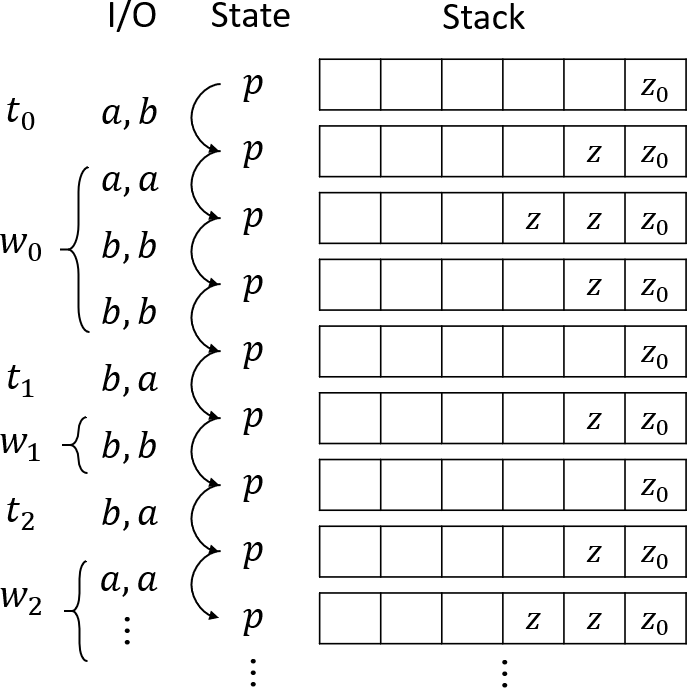
\includegraphics[width=6cm]{PDT.png}
%   \caption{An example of run for a sequence $w = t_0 w_0 t_1 w_1\cdots$.}
%   \label{fig: PDT}
% \end{figure}
% \end{example}

\subsection{Pushdown automata}

\begin{definition}
A nondeterministic {pushdown automata} (NPDA) over $\Sigma_\dblI$, $\Sigma_\dblO$ and $\Gamma$ is $\calA = (Q, Q_\dblI, Q_\dblO, q_0, z_0, \delta, c)$ where
$Q$, $Q_\dblI, Q_\dblO$ are finite sets of states such that $Q=Q_\dblI\cup Q_\dblO$ and $Q_\dblI \cap Q_\dblO = \emptyset$,
$q_0\in Q_\dblI$ is the initial state,
$z_0\in \Gamma$ is the initial stack symbol,
$c: Q \to [n]$ is the coloring function where $n\in \Nat$ is the number of priorities and
$\delta: Q \times \Sigma \times \Gamma \to \scrP(Q \times \Com(\Gamma))$ is a finite set of transition rules having one of the following forms:
\begin{itemize}
\item $(q_\dblX, a_\dblX, z) \rightarrow (q_\overX, \com)$ (input/output rules)
\item $(q_\dblX, \tau, z)\to(q'_\dblX,\com)$ ($\tau$ rules)
\end{itemize}
where $(\dblX, \overX)\in\{(\dblI, \dblO), (\dblO,\dblI)\}$,
$q_\dblX, q'_\dblX\in Q_\dblX, q_\overX\in Q_\overX, a_\dblX\in \Sigma_\dblX$, $z\in \Gamma$ and $\com\in \Com(\Gamma)$.
\end{definition}
We define $\ID_\calA= Q\times \Gamma^*$ and
the transition relation $\vdash_\calA\subseteq \ID_\calA\times (\Sigma\cup\{\tau\})\times \ID_\calA$ as
$((q,u),a,(q',u'))\in\ \vdash_\calA$ iff there exist a rule $(q, a, z) \rightarrow (q', \com) \in \delta$ and a sequence $u\in \Gamma^*$ such that $z=u(0)$ and $u'=\upds(u,\com)$.
We write $(q,u)\vdash^a_\calA(q',u')$ iff
$((q,u),a,(q',u'))\in\ \vdash_\calA$.
We define a run and the language $L(\calA)$ of $\calA$ as those of TS $\calS_\calA=(\ID_\calA, (q_0,z_0),\Sigma, \{\tau\},\vdash_\calA,c')$
where $c'((q,u))= c(q)$ for every $(q,u)\in\ID_\calA$.
% We call a PDA $\calA=(P, p_0, z_0, \delta, c)$ deterministic if $|\delta(p,a,z)|\leq 1$ for all $p\in Q, a\in\Sigma$ and $z\in\Gamma$.
We call a PDA $\calA$ deterministic if $\calS_\calA$ is deterministic.
We call $\calA$ an $m$-NPDA (or $m$-DPDA when $\calA$ is deterministic)
if $\calS_\calA$ is an $m$-TS.
We abbreviate $0$-NPDA ($0$-DPDA) as NPDA (DPDA).
% nondeterministic if the language is defined as $L_N(\calS_\calA)$,
% universal if the language is defined as $L_U(\calS_\calA)$.
Let $\DPDA$ and $\NPDA$ be the classes of DPDA and NPDA, respectively.

\begin{example}
\label{ex: PDA}
Let us consider DPDA
$\calA = (\{q,p_0,p_1\},\{q\},\{p_0,p_1\},q,z,\delta,c)$
over $\{0,1\},\{a,b\}$ and $\{z\}$ where
$c(q)=c(p_0)=c(p_1)=2$ and
$\delta = \{
(q, 0, z) \rightarrow (p_0, \skip),
(q, 1, z) \rightarrow (p_1, \skip),
(p_0, a, z) \rightarrow (q, \push(z)),
(p_0, b, z) \rightarrow (q, \push(z)),
(p_1, b, z) \rightarrow (q, \push(z))
\}$.
We can see
a pair of sequences $(\rho,w)\in \ID_\calT^\omega\times (\{0,1\}\cdot\{a,b\})^\omega$ where
$\rho=(q,z)(p_0,z)(q,zz)(p_1,zz)\cdots$ and
$w=(0a1b)^\omega$
is a run of $\calA$.
Also, we can check
$L(\calA)=(\{0a\}\cup\{0b\}\cup\{1b\})^\omega$.
\end{example}

% \begin{example}
% \label{ex: PDA}
% Let us consider DPDA
% $\calA = (\{q,q',q_a,q_b\},\{q,q'\},\{q_a,q_b\},q,z,\delta,c)$
% over $\{0,1\},\{a,b\}$ and $\{z\}$ where
% $c(q')=1$, $c(s)=2$ for $s=q,q_a,q_b$ and
% $\delta$ is defined as in Fig. \ref{fig: PDA}.
% % $\delta = \{
% % (q, 0, z) \rightarrow (q_a, \skip),
% % (q, 1, z) \rightarrow (q_b, \skip),
% % (q_a, a, z) \rightarrow (q, \push(z)),
% % (q_b, b, z) \rightarrow (q, \push(z)),
% % (q_a, b, z) \rightarrow (q', \pop),
% % (q_b, a, z) \rightarrow (q', \pop),
% % (q', 0, z) \rightarrow (q_a, \skip),
% % (q', 1, z) \rightarrow (q_b, \skip)
% % \}$.
% We can see
% a pair of sequences $(\rho,w)\in \ID_\calT^\omega\times (\{0,1\}\cdot\{a,b\})^\omega$ in Example \ref{ex: PDT},
% where $\rho=(q,z)(q,z)(q,zz)(q,zz)(q,zzz)(q,zzz)\cdots$
% and $w=(0a1b)^\omega$,
% is also a run of $\calA$.
% However, $w_1=(0a1a)^\omega$ and $w_2=0b(0a1b)^\omega$
% are not in $L(\calA)$ because
% the run $(\rho_1,w_1)$ visits $q'$ infinitely and
% the input sequence $w_2$ forces a stack of $\calA$ empty
% by reading $0b$ first.
% We call $0a$ and $1b$ push subsequences and $0b$ and $1a$ pop subsequences.
% For a sequence $w\in(\{0,1\}\cdot\{a,b\})^\infty$,
% let $\#_{push}(w)$ and $\#_{pop}(w)$ be the number of
% push and pop subsequences appearing in $w$, respectively.
% We can check
% $L(\calA)=\{w\in(\{0,1\}\cdot\{a,b\})^\omega\mid
% \#_{pop}(w)$ is finite and
% $\#_{push}(w')-\#_{pop}(w')\geq 0$
% for every subsequence $w'=w(0:m)$ of $w$ for all $m\in\Natz\}$.
% For PDT $\calT$ defined in Example \ref{ex: PDT},
% we know $L(\calT)\subseteq L(\calA)$
% because $L(\calT)=(\{0a\}\cup\{1b\})^\omega$ contains no sequence that includes a pop subsequence.
% \end{example}
% \begin{figure}[t]
%   \centering
%   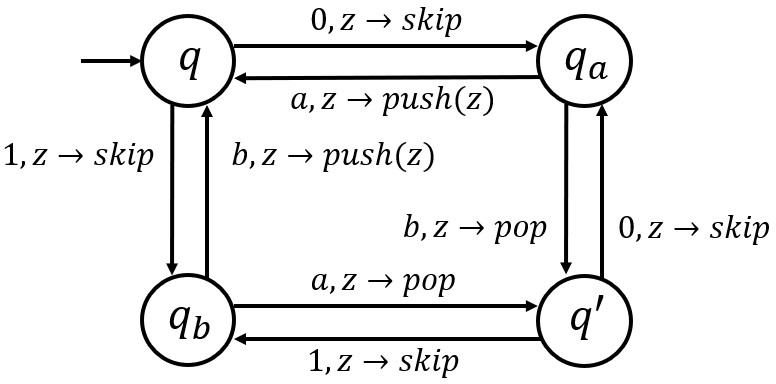
\includegraphics[width=8cm]{PDA.png}
%   \caption{States and transitions of $\calA$.
%   (A label $a,b \to c$ from $q$ to $q'$ means
%   $(q,a,b)\to(q',c)\in\delta$.)}
%   \label{fig: PDA}
% \end{figure}


The following lemma states that
the class of languages recognized by $m$-DPDA and $0$-DPDA are the same
for a fixed $m$.
\begin{lemma}
\label{lem: ef}
For a given $m$-DPDA $\calA$,
we can construct a $0$-DPDA $\calA'$ such that
$L(\calA)=L(\calA')$
\end{lemma}\
{\bf Proof sketch}\quad
We define the stack alphabet $\Gamma'$ of $\calA'$ as $\Gamma'=\Gamma^m$.
We can simulate $m$-steps with consecutive push rules (or pop rules) of $\calA$
by a single step with a push (or pop) rule of $\calA'$.

% \begin{example}
% \label{ex: PDA}
% Let us consider DPDA
% $\calA = (\{q_0,q_\bot,q_\dblI,q_\dblO\}, \{q_0,q_\dblI\}, \{q_\bot,q_\dblO\},q_0,z_0,\delta,c)$
% over $\{0,1\},\{a,b\}$ and $\{z_0,z\}$ where
% $c(q_\bot)=1$, $c(p)=2$ for $p = q_0,q_\dblI,q_\dblO$ and
% $\delta$ is defined as Fig. \ref{fig: PDA},
% in detail,
% $\delta = \{
% (p, x, z_0) \rightarrow (q_\bot, \push(z))\mid
% p\in\{q_0,q_\dblI\}, x\in\{a,b\}\}\cup
% \{(q_\bot, x, z) \rightarrow (q_\dblI, \push(z))\mid x\in\{a,b\}\}\cup
% \{(p, a, z) \rightarrow (p', \push(z)),
% (p, b, z) \rightarrow (p', \pop)\mid
% (p,p')\in\{(q_\dblI,q_\dblO), (q_\dblO,q_\dblI)\}\}$.
% For example, we can check the sequence
% $(\rho,w)\in \ID_\calT^\omega\times \{a,b\}^\omega$
% where $\rho =(q_0,z_0)(q_\bot,zz_0)(q_\dblI,zzz_0)(q_\dblO,zzzz_0)
% (q_\dblI,zzzzz_0)(q_\dblO,zzzzzz_0)\cdots$
% and $w=aba^\omega$ is a run of $\calA$.
% Because $q_\bot$ appears only one times in $\rho$,
% $w\in L(\calA)$ holds.
%
% $L(\calA)$ is the set of the sequence $w\in \{a,b\}^\omega$
% that satisfies one of the following conditions:
% (i) $w = t_0 w_0 t_1 w_1\cdots
% \in(\{ab,ba\} \times \{a,b\}^*)^\omega$
% where for all $i\geq 0$, $t_i\in \{ab, ba\}$ and
% $w_i\in \{a,b\}^*$ such that
% $\#_b(w_i)-\#_a(w_i)=2$.
% (ii) $w = t_0 w_0 t_1 w_1\cdots t_n w_n
% \in(\{ab,ba\} \times \{a,b\}^*)^*\cdot(\{ab,ba\} \times \{a,b\}^\omega)$
% where for all $0\leq i\leq n$, $t_i\in \{ab, ba\}$ and
% $w_i\in \{a,b\}^*$ such that
% $\#_b(w_i)-\#_a(w_i)=2$ for $0\leq i< n$ and
% $w_n\in \{a,b\}^\omega$ such that
% $\#_a(w')-\#_b(w')\geq 0$
% for all subsequence $w'=w(0:m)$ of $w$ for all $m\in\Natz$.
% To compare with PDT $\calT$ defined in Example \ref{ex: PDT},
% we can check $L(\calT)\subseteq L(\calA)$.
% \end{example}
% \begin{figure}[t]
%   \centering
%   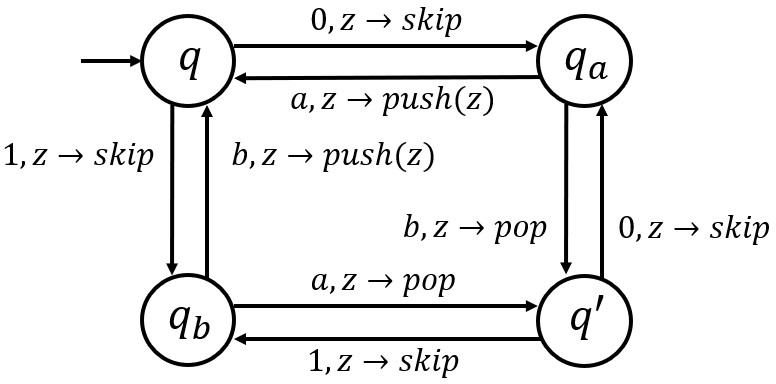
\includegraphics[width=10cm]{PDA.png}
%   \caption{States and transitions of $\calA$.
%   (A label $a,b \to c$ from $q$ to $q'$ means
%   $(q,a,b)\to(q',c)\in\delta$.)}
%   \label{fig: PDA}
% \end{figure}

\subsection{Pushdown games}

\begin{definition}
A {pushdown game} of DPDA $\calA = (Q, Q_\dblI, Q_\dblO, q_0, z_0, \delta, c)$ over $\Sigma_\dblI, \Sigma_\dblO$ and $\Gamma$ is $\calG_\calA = (V, V_\dblI, V_\dblO, E, C)$ where
$V = Q\times\Gamma^*$ is the set of vertices with $V_\dblI = Q_\dblI\times\Gamma^*, V_\dblO = Q_\dblO\times\Gamma^*$, $E\subseteq V\times V$ is the set of edges defined as $E = \{(v,v') \mid v \vdash^a v' \text{for some $a\in \Sigma_\dblI\cup\Sigma_\dblO$}\}$
and $C: V \to [n]$ is the coloring function such that
$C((q,u)) = c(q)$ for all $(q,u)\in V$.
\end{definition}

The game starts with $(q_0,z_0)\in V_\dblI$.
When the current vertex is $v\in V_\dblI$,
Player II chooses a successor $v'\in V_\dblO$ of $v$ as the next vertex.
When the current vertex is $v\in V_\dblO$,
Player I chooses a successor $v'\in V_\dblI$ of $v$.
Formally, a finite or infinite sequence $\rho\in V^\infty$ is
\emph{valid} if
$\rho(0)=(q_0,z_0)$ and
$(\rho(i-1), \rho(i))\in E$ for every $i\geq 1$.
A \emph{play} of $\calG_\calA$ is an infinite and valid sequence $\rho\in V^\omega$.
Let $\PL$ be the set of plays.
A play $\rho\in \PL$ is \emph{winning} for Player I iff
$\min\{m\in[n] \mid $ there exist an infinite
number of $i\geq 0$ such that $c(\rho(i)) = m\}$ is even.
Note that by definition, a play $\rho$ is winning for Player I iff $(\rho,w)$ is a run of $\calA$ for some $w$.

Since $\calA$ is deterministic,
the following lemma holds.
\begin{lemma}
\label{lem: cor}
Let $f_1: \PL\to(Q\times\Com(\Gamma))^\omega$ and
$f_2: (\Sigma_\dblI\cdot\Sigma_\dblO)^\omega \to \PL$ be the functions defined as follows:
\begin{itemize}
\item $f_1(\rho)=(q_0,\com_0)(q_1,\com_1)\cdots\in (Q\times\Com)^\omega$ where
$u_{i+1} = \upds(u_{i},\com_i)$
for all $i\geq 0$ and
\item $f_2(w)=\rho$ where $\rho=(q_0,u_0)(q_1,u_1)\cdots\in \PL$ and
$\rho(i)\vdash^{w(i)} \rho(i+1)$ for all $i\geq 0$.
\end{itemize}
Then, $f_1$ and $f_2$ are well-defined,
$f_1$ is an injection and $f_2(L({\cal A}))$ is the set of all the winning plays of Player I.
\end{lemma}
% {\bf Proof.}\quad
% We show both of sequences
% $\pi=(q_0,\com_0)(q_1,\com_1)\cdots\in (Q\times\Com)^\omega$
% and $w\in\Sigma^\omega$
% determinine a play
% $\rho=(q_0,u_0)(q_1,u_1)\cdots\in V^\omega$ uniquely.
% From $\pi$, we let $u\in (\Gamma^*)^\omega$ such that
% $u_0 = z_0$ and $u_{i+1} = \upds(u_{i},\com_i)$
% for all $i\geq 0$.
% Then a play
% $\rho=(q_0,u_0)(q_1,u_1)\cdots\in V^\omega$
% is determined uniquely.
% From $w$, we let a sequence $\rho\in V^\omega$
% such that there exists a run $(\rho,w)$ of $\calA$.
% Because $\calA$ is deterministic,
% $\rho$ is determined uniquely.
% \par\medskip\noindent
\begin{theorem}{\cite{Wa96}}
\label{the: wal}
If player I has a winning strategy of $\calG_\calA$,
we can construct a PDT $\calT$ over $Q_\dblI\times\Com(\Gamma), Q_\dblO\times\Com(\Gamma)$ and a stack alphabet $\Gamma'$ that gives a winning strategy of $\calG_\calA$.
That is, $\rho\in \PL$ is winning for Player I if $f_1(\rho)\in L(\calT)$.
\end{theorem}

By Lemma \ref{lem: cor},
a winning strategy can be also given as
the a subset of sequences $w\in\Sigma^\omega$
such that the play $f_2(w)$ is winning for Player I.
Thus, we can obtain the following lemma
in a similar way to Theorem \ref{the: wal}.
\begin{corollary}
\label{col: 2}
If player I has a winning strategy of $\calG_\calA$,
we can construct a PDT $\calT$ over $\Sigma_\dblI, \Sigma_\dblO$ and $\Gamma'$ that gives a winning strategy of $\calG_\calA$.
That is, $f_2(w)\in \PL$ is winning for Player I if $w\in L(\calT)$.
\end{corollary}

\section{Realizability problems for PDA and PDT}

For a specification $S$ and an implementation $I$,
we write $I \models S$ if $L(I) \subseteq L(S)$.

\begin{definition}
Realizability problem \Real ($\calS$, $\calI$) for a class of specifications $\calS$ and of implementations $\calI$: For a specification $S\in\calS$, is there an implementation $I\in\calI$ such that $I \models S$ ?
\end{definition}

\begin{example}
By Examples \ref{ex: PDT} and \ref{ex: PDA},
$L(\calT)\subseteq L(\calA)$ holds for PDT $\calT$ and DPDA $\calA$
defined in the examples.
Thus, $\calT\models\calA$ holds.
Let us consider $\calA'=(\{q_0,q_\bot,q_\dblI,q_\dblO\}, \{q_0,q_\dblI\}, \{q_\bot,q_\dblO\},q_0,z_0,\delta,c')$
which is obtained from $\calA$ but the coloring function $c'$
is defined as $c'(q_\bot)=1$ and $c'(p)=2$ for $p=q_0,q_\dblI,q_\dblO$.
For example, the pair of the sequences
$(\rho,w)\in\ID_\calA^\omega\times \Sigma^\omega$
in Example \ref{ex: PDA}
is a run of $\calA'$ but $w\notin L(\calA)$ because
$\rho$ has only one $q_\bot$ in its states.
We can check that all sequence $w'\in (\{a\}\cdot\Sigma)^\omega$
is not in $L(\calA')$ because
the run $(\rho',w')$ of $w'$ never visit $q_\bot$ over one times.
Then, we can check there are no PDT $\calT$ such that $\calT\models\calA$
because every language $L(\calT)$ of PDT $\calT$
always includes a word $w\in (\{a\}\cdot\Sigma)^\omega$,
and thus there exists a word $w\in L(\calT)\cap \overline{L(\calA)}$, it means $L(\calT)\not\subseteq L(\calA)$.
\end{example}

\begin{theorem}\label{the: DPDA}
\Real $($\DPDA, \PDT$)$ is decidable.
\end{theorem}
{\bf Proof.}\quad
Let $\calA$ be a given DPDA.
By Lemma \ref{lem: 2},
we can construct a PDT $\calT$ such that
$w\in L(T)$ iff $f^{-1}_2(w)$ is winning play of $\calG_\calA$.
By the definition of $f_2$,
$\rho(i)\vdash^{w(i)} \rho(i+1)$ holds
for all $i\geq 0$ where $\rho=f^{-1}_2(w)$.
Then, $w\in L(\calA)$ holds, and thus $\calT\models\calA$.
Hence, we can say $\calT\models\calA$ iff player I has a winning strategy for the game $\calG_\calA$.
Because there is an algorithm for constructing $\calT$
in [Walukiewucz, 2001], \Real $($\DPDA, \PDT$)$ is decidable.

% \begin{theorem}
% \Real $($\UPDA, \PDT$)$ is decidable.
% \end{theorem}
% {\bf Proof.}\quad
% For UPDA, we reduce the problem to the realizability problem for DPDA.
% W. l. o. g. assume a given UPDA $\calA = (Q, q_0, z_0, \delta, c)$ over $\Sigma_\dblI$ and $\Sigma_\dblO$ satisfies $|\delta(q,(a,b),z)|=n$ for a fixed $n\geq 2$ and
% every rule is uniquely numbered in the range of $[n]$.
% From $\calA$, we construct an DPDA $\calA' = (Q, q_0, z_0, \delta', c)$ over $\Sigma_\dblI \times [n]$ and $\Sigma_\dblO$ as the one that satisfies:
% $r = (q,(a,b),z)\to(q',Z)\in\delta$ and $r$ is numbered as $i$ iff
% $(q,((a,i),b),z)\to(q',Z)\in\delta'$.
% By the construction of $\calA'$, the following condition holds:
% \begin{eqnarray}
% (a_1,b_1)(a_2,b_2)\cdots \in L(\calA) \Leftrightarrow \nonumber\\ ((a_1,i_1),b_1)((a_2,i_2),b_2)\cdots \in L(\calA')\text{ for all }i_1,i_2,\cdots\in [n] \label{eq: upda1}
% \end{eqnarray}
%
% For a PDT $\calT=(P, p_0, z_0, \Delta)$ over $\Sigma_\dblI$ and $\Sigma_\dblO$,
% we can construct a PDT $\calT'=(P, p_0, z_0, \Delta')$ over $\Sigma_\dblI\times[n]$ and $\Sigma_\dblO$ as the one that satisfies:
% $(q,a,z)\to(q',b,Z)\in\Delta$ iff
% $(q,(a,i),z)\to(q',b,Z)\in\Delta'$ for every $i\in[n]$.
% By the construction of $\calT'$, the following condition holds:
% \begin{eqnarray}
% (a_1,b_1)(a_2,b_2)\cdots \in L(\calT) \Leftrightarrow \nonumber\\ ((a_1,i_1),b_1)((a_2,i_2),b_2)\cdots \in L(\calT')\text{ for all }i_1,i_2,\cdots\in [n] \label{eq: upda2}
% \end{eqnarray}
% by (\ref{eq: upda1}) and (\ref{eq: upda2}),
% $\calT\models\calA \Leftrightarrow \calT'\models\calA'$ holds.
% Therefore, $\exists\calT.\calT\models\calA \Leftrightarrow \exists\calT'.\calT'\models\calA'$, and the realizability problem for UPDA is decidable by this reduction.

% \begin{theorem}
% The realizability problem for PDT and DPDA is decidable.
% \end{theorem}
% {\bf Proof.}\quad
% Assume $\Sigma_\dblI = \{0,1\}$.
% We reduce the problem to emptiness problem of DPDTA.
% For an DPDA $\calA=(Q, Q_\dblI, Q_\dblO, q_0, z_0, F, \delta_\calA)$ over $\Sigma_\dblI$, $\Sigma_\dblO$ and $\Gamma$,
% we construct an DPDTA $\calB=(Q\times\Sigma_\dblO, (q_0, a_0), z_0, F\times\Sigma_\dblO, \delta_\calB)$ over $\Sigma_\dblO$ and $\Gamma$ for some $a_0\in\Sigma_\dblO$, and
% an DPDT $\calT=(Q, q_0, z_0, \Delta)$ over $\Sigma_\dblI, \Sigma_\dblO$ and $\Gamma$ as satisfying follows:
% $(p, 0, z) \to (q, z'_0), (q, a, z'_0) \to (p'_0, Z_0), (p, 1, z) \to (q, z'_1), (q, b, z'_1) \to (p'_1, Z_1)\in \delta_\calA$ iff $((p,c), c, z) \to ((p'_0, a), Z_0), ((p'_1, b), Z_1) \in \delta_\calB$ for all $c\in \Sigma_\dblO$ iff $(p, 0, z)\to (p'_0, a, Z_0), (p, 1, z)\to (p'_1, b, Z_1)\in\Delta$ iff .
%
% % Then, every transition rule of $\calB$ determines input symbols read in the child positions of input tree. Thus, $L(\calB)$ must be singleton or emptyset.
%
% Assume $L(\calB)\neq\emptyset$. Then, there exists an accepting run $(\rho,t)$ of $\calB$.
% Therefore, for every $w\in\{0,1\}^\infty$, there exists a unique run $(\rho_w,t_w)$ of $\calT$.
% Because $(\rho_w,t_w)$ is also an accepting run of $\calA$, $t_w\in L(\calT) \Rightarrow t_w\in L(\calA)$ holds for all $w$ (and also for all sequence over $\Sigma_\dblI$ and $\Sigma_\dblO$), and thus $\calT\models\calA$.
%
% Assume $L(\calB)=\emptyset$.
% Then, for every run of $\calB$, there exists $w$ such that
% the run $(\rho_w,t_w)$ of $\calA$ is not accepting.
% Thus, every PDT cannot realize $\calA$ because every run of PDT with $w$ does not accepted by $\calA$. Thus, $\calT'\not\models\calA$ for any PDT $\calT'$.
%
% Hence, $L(\calB)\neq\emptyset$ iff there exists a PDT $\calT$ such that $\calT\models\calA$.
%
% \begin{theorem}
% The realizability problem for PDT and DPDA is decidable.
% \end{theorem}
% {\bf Proof.}\quad
% Assume $\Sigma_\dblI = \{0,1\}$.
% We reduce the problem to emptiness problem of DPDTA.
% For an DPDA $\calA=(Q, Q_\dblI, Q_\dblO, q_0, z_0, F, \delta_\calA)$ over $\Sigma_\dblI$, $\Sigma_\dblO$ and $\Gamma$,
% we construct an DPDTA $\calB=(Q, q_0, z_0, F, \delta_\calB)$ over $\Sigma_\dblO^2$ and $\Gamma$ as satisfying follows:
% $(p, 0, z) \to (q, z'_0), (q, a, z'_0) \to (p'_0, Z_0), (p, 1, z) \to (q, z'_1), (q, b, z'_1) \to (p'_1, Z_1)\in \delta_\calA$ iff $(p, (a,b), z) \to (p'_0, Z_0), (p'_1, Z_1) \in \delta_\calB$.

\begin{theorem}
\label{th: NPDA-PDT}
\Real $($\NPDA, \PDT$)$ is undecidable.
\end{theorem}
{\bf Proof.}\quad
We prove the theorem by a reduction from the universality problem of NPDA, which is undecidable.
For a given NPDA $\calA = (Q, Q_\dblI, Q_\dblO, q_0, z_0, \delta, c)$ over $\Sigma_\dblI, \Sigma_\dblO$ and $\Gamma$,
we can construct an NPDA $\calA' = (Q\times[2], Q\times\{1\}, Q\times\{2\}, q_0, z_0, \delta',c')$ over $\Sigma'_\dblI, \Sigma'_\dblO$ and $\Gamma$
where $\Sigma'_\dblI = \Sigma_\dblI\cup \Sigma_\dblO$,
$\Sigma'_\dblO$ is an arbitrary (nonempty) alphabet,
$c'((q,1))=c'((q,2))=c(q)$ for all $q\in Q$
and $\delta'$ satisfies that
$((q,1),a,z)\to ((q',2),\com)\in\delta$ iff $(q,a,z)\to (q',\com)\in\delta'$, and
$((q',2),b,z)\to ((q',1),\skip)\in\delta'$ for all $b\in \Sigma'_\dblO$ and $z\in \Gamma$.

We show $L(\calA)=(\Sigma'_\dblI)^\omega$ iff there exists $\calT$ such that $\calT\models\calA$.
By the construction of $\calA'$, $L(\calA')=\<L(\calA),(\Sigma'_\dblO)^\omega\>$ holds.
If $L(\calA)=(\Sigma'_\dblI)^\omega$, then $L(\calA')=\<(\Sigma'_\dblI)^\omega,(\Sigma'_\dblO)^\omega\>$
and thus $\calT\models\calA$ holds for every $\calT$.
Assume that $L(\calA)\neq(\Sigma'_\dblI)^\omega$.
Then, there exists a word $w\in(\Sigma'_\dblI)^\omega$ such that $w\notin L(\calA)$.
For any PDT $\calT$ and any $u\in(\Sigma'_\dblI)^\omega$, there is $v\in(\Sigma'_\dblO)^\omega$ such that $\<u, v\>\in L(\calA')$.
On the other hand, $\<w, v\>\notin L(\calA')$ holds for any $v\in(\Sigma'_\dblO)^\omega$.
Hence, $\calT\not\models\calA'$ holds for any PDT $\calT$.
This completes the reduction and the realizability problem for PDT and NPDA is undecidable.

\section{Register Pushdown Transducers and Automata}
\subsection{Data words and registers}
We assume a countable set $D$ of \emph{data values}.
For finite alphabets $\Sigma_\dblI,\Sigma_\dblO$,
an infinite sequence $(a^\dblI_1,d_1)(a^\dblO,d'_1)\cdots \in ((\Sigma_\dblI\times D)\cdot(\Sigma_\dblO\times D))^\omega$ is called a \emph{data word}.
We let $\DW(\Sigma_\dblI,\Sigma_\dblO,D)=((\Sigma_\dblI\times D)\cdot(\Sigma_\dblO\times D))^\omega$.
We define the projection $\lab: \Sigma\times D \to \Sigma$ as $\lab((a,d))=a$ for $(a,d)\in \Sigma\times D$.
For $k\in\Natz$, a mapping $\theta: [k] \to D$ is called an \emph{assignment}
(of data values to $k$ registers).
Let $\Theta_k$ denote the collection of assignments to $k$ registers.
We assume $\bot\in D$ as the initial data value and
let $\theta^k_\bot\in\Theta_k$ be the initial assignment such that
$\theta^k_\bot(i)=\bot$ for all $i\in[k]$.

% For $j_1\cdots j_n\in [k]^*$, we define $\theta(j_1\cdots j_n)=\theta(j_1)\cdots\theta(j_n)$ and $\theta(\varepsilon) = \varepsilon$.
We denote $\Tst_k = \scrP([k]\cup\{\top\})$ and $\Asgn_k = \scrP([k])$
where $\top\notin\Nat$ is a unique symbol that represents a stack top value.
$\Tst_k$ is the set of guard conditions.
For $\tst\in\Tst_k$, $\theta\in\Theta_k$ and $d,e\in D$,
we denote $(\theta,d,e)\models\tst$
if ($\theta(i) = d \Leftrightarrow i\in\tst$)
and ($e = d \Leftrightarrow \top\in\tst$) hold.
In the definitions of register pushdown transducer and automaton in the next section,
the data values $d$ and $e$ correspond to an input data value and a stack top data value, respectively.
$\Asgn_k$ is the set of assignment conditions.
For $\asgn\in\Asgn_k$, $\theta\in\Theta_k$ and $d\in D$,
let $\theta[\asgn\leftarrow d]$ be the assignment
$\theta'\in\Theta_k$ such that $\theta'(i) = d$ for $i\in\asgn$ and $\theta'(i)=\theta(i)$ for $i\notin\asgn$.

\subsection{Register pushdown transducers}
\begin{definition}
A $k$-{register pushdown transducer} ($k$-RPDT) over finite alphabets $\Sigma_\dblI,\Sigma_\dblO$ and $\Gamma$ is
$\calT=(P, p_0, z_0, \Delta)$ where
$P$ is a finite set of states,
$p_0\in P$ is the initial state,
$z_0\in \Gamma$ is the initial stack symbol and
$\Delta: P\times\Sigma_\dblI\times\Tst_k\times\Gamma \to P\times\Sigma_\dblO\times \Asgn_k \times [k]\times \Com(\Gamma\times[k])$ is a finite set of deterministic transition rules.
\end{definition}
% $D$ is used as a stack alphabet.
For $u\in (\Gamma\times D)^+$, $\theta'\in\Theta_k$ and $\com\in\Com(\Gamma\times[k])$, let us define $\upds(u,\theta',\com)$ as $\upds(u,\theta',\pop)=u(1:)$, $\upds(u,\theta',\skip)=u$ and $\upds(u,\theta',\push((z,j')))=(z,\theta'(j'))u$.
Let $\ID_\calT= P\times \Theta_k\times (\Gamma\times D)^*$
and $\Rightarrow_\calT\ \subseteq \ID_\calT\times ((\Sigma_\dblI\times D)\cdot(\Sigma_\dblO\times D))\times \ID_\calT$ be the transition relation of $\calT$ such that $((p, \theta, u), (a,d^\dblI)(b,d^\dblO), (q, \theta', u'))\in\ \Rightarrow_\calT$ iff
there exists a rule $(p, a, \tst, z) \to (q, b, \asgn, j, \com) \in \Delta$
that satisfies the following conditions:
$(\theta, d^\dblI, \scnd(u(0)))\models\tst$, $\theta' = \theta[\asgn\leftarrow d^\dblI]$, $\theta'(j) = d^\dblO$,
$z=\fst(u(0))$ and
$u'=\upds(u,\theta',\com)$,
and we write $(p, \theta, u) \done_{\calT}^{(a,d^\dblI)(b,d^\dblO)}(q, \theta', u')$.
% If a sequence of IDs $(q_0, \theta_0, w_0), \cdots, (q_n, \theta_n, w_n)\in \ID_\mathcal{T}$
% and data values $d^\dblI_1, \cdots, d^\dblI_n, d^\dblO_1, \cdots, d^\dblO_n\in D$ satisfy $(q_{i-1}, \theta_{i-1}, w_{i-1})\done^{d^\dblI_i, d^\dblO_i}(q_i, \theta_i, w_i)$ for all $i\in[n]$, we write $(q_0, \theta_0, w_0)\done^{w^\dblI, w^\dblO}(q_n, \theta_n, w_n)$
% where $w^\dblI = d^\dblI_1 \cdots d^\dblI_n$ and $w^\dblO = d^\dblO_1 \cdots d^\dblO_n$.

% If we emphasize the rule $r$ and the data value $d$,
% we write $\done_d^r$.
A run and the language $L(\calT)$ of $\calT$ are those of deterministic $0$-TS $(\ID_\calT, (q_0,\theta^k_\bot, (z_0,\bot)), (\Sigma_\dblI\times D)\cdot(\Sigma_\dblO\times D), \emptyset, \Rightarrow_\calT, c)$ where $c(s)=2$ for all $s\in\ID_\calT$.
In this paper,
we assume that no run of RPDT reaches an ID whose stack is empty.
Let \RPDTk\ be the class of $k$-RPDT and \RPDT = $\bigcup_{k\in\Natz}$\RPDTk.
% Note that \RPDT$[0]$ = \PDT.

\subsection{Register pushdown automata}\label{sec:RA}
\begin{definition}
A nondeterministic $k$-register pushdown automaton ($k$-NRPDA) over $\Sigma_\dblI,\Sigma_\dblO$ and $\Gamma$ is $\calA=(Q, Q_\dblI, Q_\dblO, q_0, z_0, \delta, c)$, where
$Q$ is a finite set of states,
$Q_\dblI\cup Q_\dblO = Q, Q_\dblI\cap Q_\dblO = \emptyset$,
$q_0\in Q$ is the initial state,
$z_0\in \Gamma$ is the initial stack symbol,
$c: Q \to [n]$ where $n\in \Nat$ is the number of priorities
and
$\delta: Q \times (\Sigma\cup\{\tau\})\times \Tst_k\times\Gamma \to \scrP(Q \times\Asgn_k\times \Com(\Gamma\times[k]))$ is a transition function having one of the forms:
\begin{itemize}
\item $(q_\dblX,a_\dblX,\tst,z)\to(q_\overX,\asgn,\com)$ (input/output rule)
\item $(q_\dblX,\tau,\tst,z)\to(q'_\dblX,\asgn,\com)$ ($\tau$ rule)
\end{itemize}
where $(\dblX, \overX)\in\{(\dblI, \dblO), (\dblO,\dblI)\}$,
$q_\dblX, q'_\dblX\in Q_\dblX, q_\overX\in Q_\overX, a_\dblX\in \Sigma_\dblX$, $\tst\in\Tst_k$, $z\in\Gamma$, $\asgn\in\Asgn_k$ and $\com\in\Com(\Gamma\times[k])$.
\end{definition}
\noindent
Let $\ID_\calA= Q\times \Theta_k\times (\Gamma\times D)^*$.
We define the transition relation $\vdash_\calA\ \subseteq\ID_\calA\times ((\Sigma\cup\{\tau\})\times D)\times \ID_\calA$ as
$((q,\theta,u), (a,d), (q',\theta',u'))\in\ \vdash_\calA$,
written as $(q,\theta,u)\vdash^{(a,d)}_{\calA}(q',\theta',u')$, iff
there exists a rule $(p, a, \tst, z) \to (q, \asgn, \com) \in \delta$
such that
$(\theta, d, \scnd(u(0)))\models\tst$, $\theta' = \theta[\asgn\leftarrow d]$,
$z=\fst(u(0))$ and
$u'= \upds(u,\theta',\com)$.
For $s,s'\in\ID_\calA$ and
$w\in((\Sigma_\dblI\times D)\cdot (\Sigma_\dblO\times D))^{m}$,
we write $s\vdash^{w}s'$ if
there exists $\rho\in\ID_\calA^{m+1}$ such that
$\rho(0)=s, \rho(m)=s'$, and
$\rho(0)\vdash^{w(0)}\cdots\vdash^{w(m-1)}\rho(m)$.

A run and the language $L(\calA)$ of $k$-DRPDA $\calA$ are those of TS
$\calS_\calA=(\ID_\calA, (q_0, \theta^k_\bot, (z_0,\bot)), \Sigma\times D, \{\tau\}\times D, \vdash_\calA, c')$ where
$c'((q,\theta,u))=c(q)$ for all $(q,\theta,u)\in\ID_\calA$.
We call $\calA$ deterministic, or $k$-DRPDA, if $\calS_\calA$ is deterministic.
We call $\calA$ an $(m,k)$-NRPDA (or an $(m,k)$-DRPDA when $\calA$ is deterministic)
if $\calS_\calA$ is an $m$-TS.
We abbreviate $(0,k)$-NRPDA ($(0,k)$-DPDA) as $k$-NRPDA ($k$-DRPDA).
Let \DRPDA\ and \NRPDA\ be the unions of $k$-DRPDA and $k$-NRPDA for all $k\in\Natz$, respectively.

\medskip
For simplicity,
we assume that the set of stack alphabet $\Gamma$
is the singleton $\{z\}$.
We abbreviate
$k$-RPDT $\calT=(P, p_0, z_0, \Delta)$ as $\calT=(P, p_0, \Delta)$,
the set of all
IDs of $k$-RPDT $P\times\Theta_k\times(\Gamma\times D)^+$
as $P\times\Theta_k\times D^+$,
the stack command $\Com(\Gamma\times[k])$ as $\Com([k])$,
every rule $(p, a, \tst, z) \to (q, b, \asgn, j, \com)$ of $\calT$ as
$(p, a, \tst) \to (q, b, \asgn, j, \com')$ where
$\com\in\Com(\Gamma\times[k])$ and $\com'\in\Com([k])$
such that $\com'=\com$ if $\com=\pop$ or $\skip$ and
$\com'=\push(j')$ if $\com'=\push(z,j')$ for some $j'\in[k]$.
except in the proof of Theorem \ref{th: DPDAv}.
We apply a similar abbreviation to those of RPDA.

\begin{example}
\label{ex: RPDT}
Let us consider $1$-RPDT
$\calT = (\{p\},p,\Delta)$
over $\{a\},\{b\}$
and $\Gamma$ ($=\{z\}$) where
$\Delta = \{
(p, a, \{1,\top\}) \rightarrow (p, b, \emptyset, 1, \skip),$
$(p, a, \emptyset) \rightarrow (p, b, \{1\}, 1, \push(1))
\}$
Let $\rho=(p,[\bot],\bot)(p,[d_1],d_1\bot)(p,[d_1],d_1\bot)(p,[d_2],d_2d_1\bot)\cdots$
, $[d]\in\Theta_1$ be the assignment such that $[d](1)=d$,
and
$w=(a,d_1)(b,d_1)(a,d_1)(b,d_1)(a,d_2)(b,d_2)\cdots$,
then $(\rho,w)$ is a run of $\calT$.
\end{example}

\subsection{Visibly RPDA}
Let $\Com_v=\{\pop,\skip,\push\}$ and $v:\Com([k])\to\Com_v$ be the function such that $v(\push(j))=\push$ for $j\in[k]$ and $v(\com)=\com$ otherwise.
We say that a $k$-DRPDA $\calA$
over $\Sigma_\dblI,\Sigma_\dblO$ and $\Gamma$
visibly manipulates its stack (or a {\em stack-visibly} RPDA) if
there exists a function $\vis: \Sigma\to\Com_v$
such that
every rule $(q,a,\tst)\to(q',\asgn,\com)$ of $\calA$
satisfies $\vis(a)=v(\com)$.
We define a stack-visibly PDA in a similar way.
Stack-visibility of RPDA will be used
in the proof of Lemma \ref{lem: LkS}
in order to take the intersection of the two DRPDA.

Also, we say that $\calA$ is a {\em test-visibly} DRPDA if
there exists a function $\vis_t: \Sigma\to\Tst_k$
such that
every rule $(q,a,\tst)\to(q',\asgn,\com)$ of $\calA$
satisfies $\vis_t(a)=\tst$.
In the next subsection,
we prove that the projection of the language recognized by
a NRPDA $\calA$ onto the finite alphabets
can be recognized by a NPDA $\calA'$,
and if $\calA$ is a test-visibly DRPDA,
$\calA'$ is deterministic.

If $\calA$ is a stack-visibly and test-visibly DRPDA,
we call $\calA$ a visibly DRPDA.
Let \DRPDAv\ be the union of visibly $k$-DRPDA for all $k\in\Natz$, respectively.

\section{Realizability problems for RPDA and RPDT}
\subsection{Finite actions}
For $k\in\Natz$,
we define the set of visibly finite input actions as $A_k^\dblI = \Sigma_\dblI\times\{\skip\}\times \Tst_k$
and the set of visibly output actions as $A_k^\dblO = \{(\sigma_o, v(\com), \asgn, j, \com)\in \Sigma_\dblO\times\Com_v\times \Asgn_k\times [k]\times \Com([k])\}$ for $k$-RPDT.
A sequence $w = ((a^\dblI_0, \skip),d^\dblI_0) ((a^\dblO_0,v(\com_0)),d^\dblO_0)\cdots \in \DW(\Sigma_\dblI,\Sigma_\dblO,D)$ is compatible with a sequence
$\overa = (a^\dblI_0, \skip,\tst_0)(a^\dblO_0,v(\com_0),\asgn_0,j_0, \com_0)\cdots \in (A_k^\dblI\cdot A_k^\dblO)^\omega$
iff there exists a sequence $(\theta_0,u_0)(\theta_1, u_1)\cdots\in (\Theta_k\times D^*)^\omega$, called \emph{witness}, such that
$\theta_0 = \theta_\bot$, $u_0 = \bot$,
$\theta_i, d^\dblI_i, u_i(0) \models \tst_i, \theta_{i+1}=\theta_i[\asgn_i\leftarrow d^\dblI_i], \theta_{i+1}(j_i) = d^\dblO_i$ and $u_{i+1}={u_i(1:)}, u_i, \theta_{i+1}(j')u_i$
if $\com_i=\pop,\skip,\push(j')$, respectively.
Let $\Comp(\overa) = \{w\in \DW(\Sigma_\dblI,\Sigma_\dblO,D)\mid$ $w$ is compatible with $\overa$ $\}$.
For specification $S \subseteq \DW(\Sigma_\dblI\times\Com_v,\Sigma_\dblO\times\Com_v,D)$, we define $W_{S,k}=\{\overa\mid \Comp(\overa)\subseteq S\}$.

For a data word $w\in\DW(\Sigma_\dblI,\Sigma_\dblO,D)$ and
a sequence $\overa\in(A_k^\dblI\cdot A_k^\dblO)^\omega$
such that $w(i)=(a,d)$ and $\overa(i)=(a,\cdot)$ for all $i\geq 0$,
we define $w\otimes\overa\in\DW(A_k^\dblI,A_k^\dblO,D)$ as satisfying
$w\otimes\overa(i)=(\overa(i), d)$ where $w(i)=(a,d)$.

\begin{theorem}\label{the: finite_actions}
For a specification $S\subseteq \DW(\Sigma_\dblI\times\Com_v,\Sigma_\dblO\times\Com_v,D))$, the following statements are equivalent.
\begin{itemize}
\item There exists a $k$-RPDT $\calT$ such that $L(\calT)\subseteq S$.
\item There exists a PDT $\calT'$ such that $L(\calT')\subseteq W_{S,k}$.
\end{itemize}
\end{theorem}

\subsection{Decidability and undecidability of realizability problems}
\begin{lemma}\label{lem: Lk}
$L_k = \{w\otimes\overa \mid w\in\Comp(\overa)\}$ is definable as a language of $(2,k+2)$-DRPDA.
\end{lemma}
{\bf Proof.}\quad
Let $(2,k+2)$-DRPDA $\calA_k = (\{p, q\}\cup(\Asgn_k\times[k]\times\Com([k]))\cup[k], \{p\}, \{q\}\cup(\Asgn_k\times[k]\times\Com([k]))\cup[k], p, \delta_k, c_k)$ over $A_k^\dblI, A_k^\dblO$ and $D$ where
$c_k(s)=2$ for all state $s$ and $\delta_k$ consists of rules of the form
\begin{eqnarray}
(p, (a_\dblI, \skip, \tst), \tst\cup\tst') &\to& (q, \{k+1\}, \skip)\label{eq: Lk1}\\
(q, (a_\dblO, v(\com), \asgn, j, \com), \tst'')&\to& ((\asgn,j,\com), \{k+2\},\skip)\label{eq: Lk2}\\
((\asgn,j,\com), \tau, \{k+1\}\cup\tst'')&\to& (j, \asgn, \com)\label{eq: Lk3}\\
(j, \tau, \{j, k+2\}\cup\tst'')&\to& (p, \emptyset, \skip)\label{eq: Lk4}
\end{eqnarray}
for all $(a_\dblI, \tst)\in A_k^\dblI$, $(a_\dblO, \asgn, j, \com)\in A_k^\dblO$, $\tst'\subseteq \{k+1,k+2\}$ and $\tst''\in\Tst_{k+2}$.

We show $L(\calA_k) = L_k$.
For this proof, we redefine compatibility for finite sequences $w\in ((\Sigma_\dblI\times D)\cdot (\Sigma_\dblO\times D))^*$ and $\overa\in(A_k^\dblI\cdot A_k^\dblO)^*$.
We show the following claim.
\par\medskip\noindent
{\it Claim.} Assume $n\in\Natz$ and let $w\otimes\overa = ((a^\dblI_0, \skip,\tst_0), d^\dblI_0)((a^\dblO_0,v(\com_0),\asgn_0,j_0, \com_0), d^\dblO_0)\cdots\in ((A_k^\dblI\times D)\cdot(A_k^\dblO\times D))^*$
whose length is $2n$ and
$\rho = (\theta_0,u_0)(\theta_1, u_1)\cdots\in (\Theta_k\times D^*)^*$ whose length is $n+1$ and $(\theta_0, u_0)=(\theta_\bot, \bot)$.
Then,
$\rho$ is a witness of the compatibility between $w$ and $\overa$ iff
$(p,\theta'_0,u_0)\vdash^{w\otimes\overa(0:1)(\tau,d^\dblI_{0})(\tau,d^\dblO_{0})}(\theta'_1,u_1)\vdash^{w\otimes\overa(2:3)(\tau,d^\dblI_{1})(\tau,d^\dblO_{1})}\cdots\vdash^{w\otimes\overa(2n-2:2n-1)(\tau,d^\dblI_{n-1})(\tau,d^\dblO_{n-1})}(p,\theta'_{n},u_{n})$
where $\theta'_i\in \Theta_{k+2}$ ($i\in[n]$) satisfies $\theta'_i(j)=\theta_i(j)$ for $j\in[k]$.
\par\medskip\noindent
(Proof of the claim)
We show the claim by induction on $n$.
The case of $n=0$ is obvious.
We show the claim for arbitrary $n>0$ with the induction hypothesis.

We first show left to right.
By the induction hypothesis,
$(p,\theta'_0,u_0)\vdash^{w\otimes\overa(0:1)(\tau,d^\dblI_{0})(\tau,d^\dblO_{0})\cdots w\otimes\overa(2n-4:2n-3)(\tau,d^\dblI_{n-2})(\tau,d^\dblO_{n-2})}(p,\theta'_{n-1},u_{n-1})$ holds.
By the assumption, because $\rho$ is the witness,
(a) $\theta_{n-1}, d^\dblI_{n-1}, u_{n-1}(0) \models \tst_{n-1}$,
(b) $\theta_{n}=\theta_{n-1}[\asgn_{n-1}\leftarrow d^\dblI_{n-1}]$,
(c) $\theta_{n}(j_{n-1}) = d^\dblO_{n-1}$ and
(d) $u_{n}={u_{n-1}(1:)}, u_{n-1}, \theta_{n}(j')u_{n-1}$
if $\com_{n-1}=\pop,\skip,\push(j')$, respectively.
By the condition (a),
$\calA_k$ can do a transition
$(p,\theta'_{n-1},u_{n-1})\vdash^{w\otimes\overa(2n-2)}
(q,\theta^1_{n-1},u_{n-1})$ for unique $\theta^1_{n-1}\in\Theta_{k+2}$ by the rule $(p, (a^\dblI_{n-1}, \skip, \tst_{n-1}), \tst_{n-1}\cup\tst') \to (q, \{k+1\}, \skip)$ of the form (\ref{eq: Lk1}).
We can also say
$(q,\theta^1_{n-1},u_{n-1})\vdash^{w\otimes\overa(2n-1)}
((\asgn_{n-1}, j_{n-1}, \com_{n-1}),\theta^2_{n-1},u_{n-1})$ by the rule of the form (\ref{eq: Lk2}). Note that $\theta^2_{n-1}(j)=\theta_{n-1}(j)$ if $j\in[k]$, $\theta^2_{n-1}(k+1)=d^\dblI_{n-1}$ and
$\theta^2_{n-1}(k+2)=d^\dblO_{n-1}$.
$((\asgn_{n-1}, j_{n-1}, \com_{n-1}),\theta^2_{n-1},u_{n-1})\vdash^{(\tau,d^\dblI_{n-1})}(j_{n-1},\theta^3_{n-1},u_{n})$ is also valid transition of $\calA_k$ of the form (\ref{eq: Lk3}) by the conditions (b) and (d)
where $\theta_3^{n-1}(j)=\theta_{n}(j)$
for $j\in[k]$ and $\theta^3_{n-1}(k+2)=d^\dblO_{n-1}$.
By the condition (c), $\theta_3^{n-1}(j_{n-1})=\theta_3^{n-1}(k+1)=d^\dblO_{n-1}$ holds.
Thus, a transition $(j_{n-1},\theta^3_{n-1},u_{n})\vdash^{(\tau,d^\dblO_{n-1})}(p,\theta'_{n},u_{n})$ is valid with the rule of the form (\ref{eq: Lk4}).
In conclusion,
$(p,\theta'_{n-1},u_{n-1})\vdash^ {w\otimes\overa(2n-2:2n-1)(\tau,d^\dblI_{n-1})(\tau,d^\dblO_{n-1})}(p,\theta'_{n},u_{n})$
holds, and with the induction hypothesis, we obtain the left to right of the claim.

Next, we prove right to left. By the assumption,
$(p,\theta'_{n-1},u_{n-1})\vdash^ {w\otimes\overa(2n-2:2n-1)(\tau,d^\dblI_{n-1})(\tau,d^\dblO_{n-1})}(p,\theta'_{n},u_{n})$
holds. By checking four transition rules that realize the above transition relation, we can obtain that $\rho(n-1), \rho(n), w\otimes\overa(2n-2)$ and $w\otimes\overa(2n-1)$ satisfies the conditions (a) to (d) described in the previous paragraph. Thus, by the induction hypothesis,
we obtain $\rho$ is a witness of the compatibility between $w$ and $\overa$.
\par\medskip\noindent
\begin{flushright}
(end of the proof of the claim)
\end{flushright}
\par\medskip\noindent
By the claim,
$w\otimes\overa \in L_k\Leftrightarrow$
there exists a witness $(\theta_0,u_0)(\theta_1, u_1)\cdots\in (\Theta_k\times D^*)^\omega$ of $w$ and $\overa\Leftrightarrow$
there exists a run
$(p,\theta'_0,u_0)\vdash^{w\otimes\overa(0:1)(\tau,d^\dblI_{0})(\tau,d^\dblO_{0})}(\theta'_1,u_1)\vdash^{w\otimes\overa(2:3)(\tau,d^\dblI_{1})(\tau,d^\dblO_{1})}\cdots$ of $\calA\Leftrightarrow$
$w\otimes\overa \in L(\calA_k)$ holds.

\begin{lemma}\label{lem: LkS}
For specification $\calS$ definable by some visibly $\varepsilon$-free $k'$-DRPDA.
$L_{k, \overS} = \{w\otimes\overa \mid w\in\Comp(\overa)\cap \overS\}$
is definable as a language of visibly $(4,k+k'+4)$-DRPDA.
\end{lemma}
{\bf Proof.}\quad
Let $L_{\overS} = \{w\otimes\overa\mid w\in\overS\}$,
$\calA_{\overS}$ be a visibly $\varepsilon$-free $k'$-DRPDA such that $L(\calA_{\overS})= L_{\overS}$ and $\calA_k$ be a $(2,k+2)$-DRPDA defined in Lemma \ref{lem: Lk}.
Because $L_{k, \overS} = L_k \cap L_{\overS}$ and both $L_k$ and $L_{\overS}$ are
visibly DRPDA, it is enough to show we can construct visibly $(4,k+k'+4)$-DRPDA $\calA$ such that $L(\calA)=L(\calA_{\overS})\cap L(\calA_k)$.

For simplicity, we rewrite $\calA_k$ as $(2,k_1)$-DRPDA $\calA_1=(Q_1, Q^\dblI_1, Q^\dblO_1, q^0_1, \delta_1, c_1)$ and $\calA_{\overS}$ as $k_2$-DRPDA $\calA_2=(Q_2, Q^\dblI_2, Q^\dblO_2, q^0_2, \delta_2, c_2)$, but they satisfy that $c_1(q)$ is even for all $q\in Q_1$ and
every rules in $\delta_1$ forms triple sequencial rules
\begin{align}
(q_1, (a,v(\com_1)), \tst_1) &\to (q_2,\asgn_1, \skip)& \tag{\ref{eq: Lk2}'}\\
(q_2, \tau, \tst_2) &\to (q_3,\asgn_2, \com_1)& \tag{\ref{eq: Lk3}'}\\
(q_3, \tau, \tst_3) &\to (q_4,\asgn_3, \skip)& \tag{\ref{eq: Lk4}'}.
\end{align}
Note that $(\ref{eq: Lk2}'), (\ref{eq: Lk3}')$ and $(\ref{eq: Lk4}')$ correspond to $(\ref{eq: Lk2}), (\ref{eq: Lk3})$ and $(\ref{eq: Lk4})$, respectively, and $(\ref{eq: Lk1})$ can be devided in three rules of the form $(\ref{eq: Lk2}'), (\ref{eq: Lk3}')$ and $(\ref{eq: Lk4}')$.

We construct $(4,k_1+k_2+2)$-DRPDA
$\calA=(Q_1\times Q_2\times[5], Q^\dblI_1\times Q^\dblI_2\times[5], Q^\dblO_1\times Q^\dblO_2\times[5], (q^1_0, q^2_0, 1), \delta, c)$
where $c((q_1,q_2,i))=c_2(q_2)$ for all $(q_1,q_2,i)\in Q$.
For all rules
\begin{itemize}
\item $(q_1, (a,v(\com_1)), \tst_1)\to(q_2,\asgn_1, \skip)$,
\item $(q_2, \tau, \tst_2)\to(q_3,\asgn_2, \com_1)$,
\item $(q_3, \tau, \tst_3)\to(q_4,\asgn_3, \skip)\in\delta_1$ and
\item $(q, (a,v(\com)), \tst)\to(q',\asgn, \com)\in\delta_2$
\end{itemize}
$(v(\com_1)=v(\com))$ for $a\in\Sigma$,
let $\tst^{+ k_1}=\{i+k_1\mid i\in\tst\}\cup\{\top\mid\top\in\tst\setminus[k_1]\}, \asgn^{+ k_1}=\{i+k_1\mid i\in\asgn\}$ and $\com^{+ k_1} = \push(j+k_1)$ if $\com=\push(j)$ and $\com^{+ k_1} = \com$ otherwise, then $\delta$ consists of the rules
\begin{itemize}
\item $((q_1, q, 1), \tau, \tst'\cup\{\top\})\to((q_1, q, 2), \{k_1+k_2+1\}, \pop)$
\item $((q_1, q, 2), \tau, \tst'\cup\{\top\})\to((q_1, q, 3), \{k_1+k_2+2\}, \push(k_1+k_2+1))$
\item $((q_1, q, 3), (a,v(\com_1)), (\tst_1\cup\tst^{+ k_1})\setminus\top\cup\{k_1+k_2+t\mid$ $t=1$ if $\top\in\tst_1$ and $t=2$ if $\top\in\tst$ $\})\to((q_2, q', 4), \asgn_1\cup\asgn^{+ k_1}, \com^{+ k_1})$
\item $((q_2, q', 4), \tau, \tst_2\cup\tst')\to((q_3, q', 5), \asgn_2, \com_1)$
\item $((q_3, q', 5), \tau, \tst_3\cup\tst')\to((q_4, q', 0), \asgn_3, \skip)$
\end{itemize}
for all $\tst'\in\Tst_{k_1+k_2+2}$.
Then, $L(\calA)=L(\calA_1)\cap L(\calA_2)$.

\begin{lemma}  \label{lem: W=lab}
$W_{S,k} = \overline{\lab(L_{\overS,k})}$.
\end{lemma}
{\bf Proof.}\quad
For every $\overa\in(A_k^\dblI A_k^\dblO)^\omega$,
$\overa\notin W_{S,k} \Leftrightarrow \Comp(\overa)\not\subseteq S
\Leftrightarrow \exists w. w\in \Comp(\overa)\cap \overS
\Leftrightarrow \exists w. w\otimes\overa\in L_{\overS,k}
\Leftrightarrow \overa\in\lab(L_{\overS,k})$.
Thus, $W_{S,k} = \overline{\lab(L_{\overS,k})}$ holds.

\begin{theorem}
For all $k\geq 0$, \Real $($\DRPDAv, \RPDTk$)$ is decidable.
\end{theorem}
{\bf Proof.}\quad
By Lemma \ref{lem: LkS}, $L_{\overS,k}$ is definable by some visibly DRPDA.
Because every language recognized by some visibly DRPDA can be converted to
the language of visibly DPDA by taking a projection on its label,
$W_{S,k}$ is definable by some visibly DPDA by Lemma \ref{lem: W=lab}.
By Theorem \ref{the: finite_actions}, we can check \Real $($\DPDA, \PDT$)$ for $W_{S,k}$, which is shown to be decidable in Theorem \ref{the: DPDA}, instead of checking \Real $($\DRPDAv, \RPDTk$)$.
% By Theorem \ref{the: finite_actions}, we can check \Real $($\UPDA, \PDT$)$ for $W_{S,k}$ instead of checking \Real $($\URPDA, \RPDTk$)$.

\begin{theorem}
For all $k\geq 0$, \Real $($\NRPDA, \RPDTk$)$ is undecidable.
\end{theorem}
{\bf Proof.}\quad
We can easily reduce the problem from \Real $($\NPDA, \PDT$)$,
whose undecidability is proved in Theorem \ref{th: NPDA-PDT}.


% \section{Realizability problems for Register Automata}
% \subsection{Finite actions}
% For $k\in\Natz$,
% we define the set of finite input actions $A_k^\dblI = \Sigma_\dblI\times \Tst_k$
% and finite output actions $A_k^\dblO = \Sigma_\dblO\times \Asgn_k\times [k]\times \Com([k])$ for $k$-RPDT.
% A sequence $w = (a^\dblI_1,d^\dblI_1) (a^\dblO_1,d^\dblO_1) \cdots \in \DW(\Sigma_\dblI,\Sigma_\dblO,D)$ is compatible with a sequence
% $\overa = (a^\dblI_1,\tst_1)(a^\dblO_1,\asgn_1,j_1, \com_1)\cdots \in (A_k^\dblI A_k^\dblO)^\omega$
% if there exists a run $(\rho, w)$ of $k$-RPDT satisfying follows:
% For all $i\geq 1$, let $\rho(i-1)=(q,\theta,eu)$ and $\rho(i)=(q',\theta',u'u)$
% for some $e\in D, u\in D^*$ and $u'\in D^*$.
% Then $\theta, d^\dblI_i, e\models \tst_i, \theta'=\theta[\asgn_i\leftarrow d^\dblI_i], \theta'(j_1) = d^\dblO_i$ and $u'=Z_D(\com,\theta',e)$ hold.
% Let $\Comp(\overa) = \{w\in \DW(\Sigma_\dblI,\Sigma_\dblO,D)\mid$ $w$ is compatible with $\overa$ $\}$.
% For specification $S \subseteq \DW(\Sigma_\dblI,\Sigma_\dblO,D)$, we define $W_{S,k}=\{\overa\mid \Comp(\overa)\subseteq S\}$.
%
% \begin{theorem}\label{the: finite_actions}
% For a specification $S\subseteq \DW(\Sigma_\dblI,\Sigma_\dblO,D)$, the following statements are equivalent.
% \begin{itemize}
% \item There exists a $k$-RPDT $\calT$ such that $L(\calT)\subseteq S$.
% \item There exists a PDT $\calT'$ such that $L(\calT')\subseteq W_{S,k}$.
% \end{itemize}
% \end{theorem}
%
% % As $A_k^\dblI$ and $A_k^\dblO$,
% % we define the set of finite input actions
% % $\dblA_k^\dblI = \Sigma_\dblI\times \Tst_k\times\Asgn_k\times \Com([k])$
% % and finite output actions
% % $\dblA_k^\dblO = \Sigma_\dblO\times \Tst_k\times\Asgn_k\times \Com([k])$ for $k$-RPDA.
% % A sequence $w = (a^\dblI_1,d^\dblI_1) (a^\dblO_1,d^\dblO_1) \cdots \in \DW(\Sigma_\dblI,\Sigma_\dblO,D)$ is compatible with a sequence
% % $\overa = (a^\dblI_1,\tst_1,\asgn_1,\com_1)(a^\dblO_1,\tst'_1,\asgn'_1,\com'_1)\cdots \in (\dblA_k^\dblI \dblA_k^\dblO)^\omega$
% % if there exists a run $(\rho, w)$ of $k$-RPDA along with conditions appearing in $\overa$.
% % Let $\Comp'(\overa) = \{w\in \DW(\Sigma_\dblI,\Sigma_\dblO,D)\mid$ $w$ is compatible with $\overa$ $\}$.
%
% \subsection{Decidability and undecidability of realizability problems}
% \begin{lemma}
% $L_k = \{w\otimes\overa \mid w\in\Comp(\overa)\}$ is definable as a language of
% $\varepsilon$-equipped $(k+1)$-DRPDA.
% \end{lemma}
% {\bf Proof.}\quad
% Let $\varepsilon$-equipped $(k+1)$-DRPDA $\calA_k = (\{p, q\}\cup(\Asgn_k\times\Com([k])), \{p\}, \{q\}\cup(\Asgn_k\times\Com([k])), p, \delta_k, c_k)$ over $A_k^\dblI, A_k^\dblO$ and $D$ where
% $c_k(s)=2$ for all state $s$ and $\delta_k$ consists of rules of the form
% $(p, (a_\dblI, \tst), \tst) \to (q, \{k+1\}, \skip)$,
% $(q, (a_\dblO, \asgn, j, \com), \tst'\cup\{j\})\to ((\asgn,\com), \emptyset,\skip)$ and
% $((\asgn,\com), \tau, \tst''\cup\{k+1\})\to (p, \asgn, \com)$
% for all $(a_\dblI, \tst)\in A_k^\dblI$, $(a_\dblO, \asgn, j, \com)\in A_k^\dblO$ and $\tst',\tst''\in\Tst_k$.
% Then, $L(\calA_k) = L_k$ holds.
%
% % {\bf Proof.}\quad
% % Let $k$-DRPDA $\calA_k = (\{p\}\cup\Asgn_k, \{p\}, \Asgn_k, p, \delta_k, c_k)$ over $A_k^\dblI, A_k^\dblO$ and $D$ where
% % $c_k(p) = c_k(p') = 2$ and $\delta_k$ consists of rules of the form
% % $(p, (a_\dblI, \tst), \tst) \to (\asgn, \asgn, \skip)$ and
% % $(\asgn, (a_\dblO, \asgn, j, \com), \{j\})\to (p, \emptyset, \com)$ for all $(a_\dblI, \tst)\in A_k^\dblI$ and $(a_\dblO, \asgn, j, \com)\in A_k^\dblO$.
% % Then, $L(\calA_k) = L_k$ holds.
%
% % \begin{lemma}\label{lab: LkS}
% % For specification $\calS$ definable by some $k'$-DRPDA.
% % $L_{k, \overS} = \{w\otimes\overa \mid w\in\Comp(\overa)\cap \overS\}$
% % is definable as a language of $\max(k,k')$-DRPDA.
% % \end{lemma}
% % {\bf Proof.}\quad
% % Assume $\calA = (Q, Q_\dblI, Q_\dblO, q_0, \delta, c)$ be a $k'$-NRPDA over $\Sigma_\dblI, \Sigma_\dblO$ and $D$ whose language equals to $\overS$.
% % Let $K = \max(k,k')$ and $\calA_{\overS,k} = (Q_\dblI\cup(Q\dblO\times\Asgn_k), Q_\dblI, Q_\dblO\times\Asgn_k, q_0, \delta', c')$ be an $K$-DRPDA over $A_K^\dblI, A_K^\dblO$ and $D$ where $c'(q)=c(q)$ for $q\in Q_\dblI$, $c'((q,\asgn))=c(q)$ for $q\in Q_\dblO$ and
% % $\delta' = \{(q, (a_\dblI, \tst), \tst) \to ((q',\asgn), \asgn, \skip)\mid (q, a_\dblI, \tst) \to (q', \asgn, \skip)\in \delta\} \cup
% % \{((q',\asgn), (a_\dblO, \asgn, j, \com), \{j\})\to (q, \emptyset, \com)\mid (q', a_\dblO, \{j\})\to (q, \emptyset, \com)\in \delta\}$.
%
% \begin{lemma}\label{lab: LkS}
% For specification $\calS$ definable by some $k'$-DRPDA.
% $L_{k, \overS} = \{w\otimes\overa \mid w\in\Comp(\overa)\cap \overS\}$
% is definable as a language of $\max(k,k')$-DRPDA.
% \end{lemma}
%
% We prove $L(\calA_{\overS,k}) = L_{\overS,k}$.
%
% \begin{lemma}  \label{lem: W=lab}
% $W_{S,k} = \overline{\lab(L_{\overS,k})}$.
% \end{lemma}
% {\bf Proof.}\quad
% For every $\overa\in(A_k^\dblI A_k^\dblO)^\omega$,
% $\overa\notin W_{S,k} \Leftrightarrow \Comp(\overa)\not\subseteq S
% \Leftrightarrow \exists w. w\in \Comp(\overa)\cap \overS
% \Leftrightarrow \exists w. w\otimes\overa\in L_{\overS,k}
% \Leftrightarrow \overa\in\lab(L_{\overS,k})$.
% Thus, $W_{S,k} = \overline{\lab(L_{\overS,k})}$ holds.
%
% \begin{theorem}
% For all $k\geq 0$, \Real $($\DRPDA, \RPDTk$)$ is decidable.
% \end{theorem}
% {\bf Proof.}\quad
% By Lemma \ref{lab: LkS}, $L_{\overS,k}$ is definable by some DRPDA.
% Because every language recognized by some NRPDA can be converted to
% the language of NPDA by taking a projection on its label,
% $W_{S,k}$ is definable by some UPDA by Lemma \ref{lem: W=lab}.
% By Theorem \ref{the: finite_actions}, we can check \Real $($\DPDA, \PDT$)$ for $W_{S,k}$, which is shown to be decidable in Theorem \ref{the: DPDA}, instead of checking \Real $($\DRPDA, \RPDTk$)$.

\section{Conclusion}
We have discussed the realizability problem
whose specification and implementation are
DPDA (NPDA) and PDT in Section 4.
By using the result in \cite{Wa96},
we show \Real$($\DPDA,\PDT$)$ is decidable.
We also show the undecidability of \Real$($\NPDA,\PDT$)$
by a reduction from the universality problem of NPDA.
In Section 5, we have defined RPDT, RPDA and
showm a way to recognize the label of the language of RPDA by PDA.
We have introduced the notions of stack-visibly \cite{AM04} and
test-visibly to discuss the decidability of realizability
for RPDA and RPDT.
We show that the behavior of registers and stack of RPDT
can be simulated by the finite alphabels defined as finite actions,
and prove that \Real$($\DRPDAv,\RPDTk$)$ can be reduced to \Real$($\DPDA,\PDT$)$.

It is still unknown whether the realizability problem is decidable
in several cases such as
the specification is given by a universal PDA,
DRPDA has no restriction on visibility and
the number of registers of RPDT is not given.
Investigating these cases are future work.


%\input{acknowledgements}
%\newpage
%\bibliographystyle{splncs04}
%\bibliography{rcfg}
\begin{thebibliography}{99}
\bibitem{AM04} R. Alur and P. Madhusudan, Visibly pushdown languages,
36th ACM Symp. Theory of Computing (STOC 2004).

\bibitem{BCJ18} R. Bloem, K. Chatterjee and B. Jobstmann, Graph Games and Reactive Synthesis,
E. M. Clarke et al. (eds.), Handbook of Model Checking, Chapter 27, 921--962, Springer, 2018.

\bibitem{BDMSS11} % [8] of WRA
M. Boja\'{n}czyk, C. David, A. Muscholl, T. Schwentick and L. Segoufin,
Two-variable logic on data words,
ACM Trans. Computational Logic 12(4), 2011.

\bibitem{BKL14}
M. Boja\'{n}czyk, B. Klin, S. Lasota,
Automata theory in nominal sets,
Logical Methods in Computer Science, 10(3:4), 1--44, 2014.

\bibitem{BCGK12}
B. Bollig, A. Cyriac, P. Gastin and K. N. Kumar,
Model checking languages of data words,
15th Int. Conf. Foundations of Software Science and Computation Structures
(FoSSaCS 2012), 391--405. %, 2012.

\bibitem{BEM97}
A. Bouajjani, J. Esparza and O. Maler,
Reachability analysis of pushdown automata: Application to model-checking,
%CONCUR 1997,
8th Int. Conf. on Concurrency Theory (CONCUR 1997),
135--150.
%, 1997,
%https://doi.org/10.1007/3-540-63141-0\_10.

\bibitem{Bo02} % [11] of WRA
P. Bouyer,
A logical characterization of data languages,
Inform. Process. Lett. 84(2), 75--85, 2002.

\bibitem{BL69} J. R. B\"{u}chi and L. H. Landweber, Solving sequential conditions by finite-state strategies,
Trans. American Mathematical Society 138, 295--311, 1969.

\bibitem{CLTW17}
Y-F. Chen, O. Leng\'{a}l, T. Tan and Z. Wu,
Register automata with linear arithmetic,
32nd Annual ACM/IEEE Symp. on Logic in Computer Science (LICS 2017).

\bibitem{CK98} % [2]
E. Y. C. Cheng and M. Kaminski,
Context-free languages over infinite alphabets,
Acta Informatica 35, 245--267, 1998.

\bibitem{CGP01}
E. M. Clarke, O. Grumberg and D. A. Peled, Model checking. MIT Press, 2001.
%2017.

\bibitem{CL15}
L. Clemente and S Lasota,
Reachability analysis of first-order definable pushdown systems,
24th EACSL Annual Conf. on Computer Science Logic (CSL 2015), 244--259. %, 2015.

\bibitem{DFSS19}
L. D'Antoni, T. Ferreira, M. Sammartino and A. Silva,
Symbolic register automata,
31th Int. Conf. on Computer Aided Verification (CAV 2019).
%LNCS 11561, 2019.

\bibitem{DL09} % [3] %% [16] of RPQd
S. Demri and R. Lazi\'{c},
LTL with freeze quantifier and register automata,
ACM Trans. on Computational Logic 10(3), 2009.

\bibitem{DLN07} % [17] of RPQd
S. Demri, R. Lazi\'{c} and D. Nowak,
On the freeze quantifier in constraint LTL: Decidability and complexity,
Inform. Comput. 205(1), 2--24, 2007.

\bibitem{ESK14} R. Ehlers, S. A. Seshia and H. Kress-Gazit, Synthesis with identifiers,
15th Int. Conf. on Verification, Model Checking, and Abstract Interpretation (VMCAI 2014), 415--433.

\bibitem{EHRS00}
J. Esparza, D. Hansel, P. Rossmanith and S. Schwoon,
Efficient algorithms for model checking pushdown systems,
%CAV 2000,
12th Int. Conf. on Computer Aided Verification (CAV 2000), 232--247. %, 2000.

\bibitem{EKS01}
J. Esparza, A. Ku\v{c}era, S. Schwoon,
Model checking LTL with regular valuations for pushdown systems,
Inform. and Comput, 186(2), 355--376, 2003.

\bibitem{EFR19} L. Exibard, E. Filiot and P.-A. Reynier, Synthesis of data word transducers,
30th Int. Conf. on Concurrency Theory (CONCUR 2019).

\bibitem{Gr67}
S. A. Greibach,
A note on pushdown store automata and regular systems,
Proc. the American Mathematical Society 18, 263--268, 1967.

\bibitem{KF94} % [4]
M. Kaminski and N. Francez,
Finite-memory automata,
Theoret. Comput. Sci. 134, 322--363, 1994.

\bibitem{KK19} A. Khalimov and O. Kupferman, Register-bounded synthesis,
30th Int. Conf. on Concurrency Theory (CONCUR 2019).

\bibitem{KMB18} A. Khalimov, B. Maderbacher and R. Bloem, Bounded synthesis of register transducers,
16th Int Symp on Automated Technology for Verification and Analysis (ATVA 2018), 494--510.

\bibitem{LTV15} % [7]
L. Libkin, T. Tan and D. Vrgo\v{c},
Regular expressions for data words,
J. Computer and System Sciences 81(7), 1278--1297, 2015.

\bibitem{LV12} % [8]
L. Libkin and D. Vrgo\v{c},
Regular path queries on graphs with data,
15th Int. Conf. on Database Theory (ICDT 2012), 74--85.

\bibitem{MRT17}
A. S. Murawski, S. J. Ramsay and N. Tzevelekos:
Reachability in pushdown register automata,
J. Computer and System Sciences 87, 58--83, 2017.

\bibitem{NSV04} % [28] of WRA
F. Neven, T. Schwentick and V. Vianu,
Finite state machines for strings over infinite alphabets,
ACM Trans. on Computational Logic 5(3), 403--435, 2004.

\bibitem{PR89} A. Pnueli and R. Rosner, On the synthesis of a reactive module,
16th ACM Symp. on Principles of Programming Languages (POPL 1989), 179--190.

\bibitem{RBB10}
J. Rot, F. de Boer and M. Bonsangue,
Pushdown system representation for unbounded object creation,
Tech. Rep. KIT-13, Karlsruhe Institute of Technology, 38--52, 2010.

\bibitem{Se06} % [10] %% [40] of RPQd
L. Segoufin,
Automata and logics for words and trees over an infinite alphabet,
15th EACSL Annual Conf. on Computer Science Logic (CSL 2006), 41--57.

\bibitem{STS18} R. Senda, Y. Takata and H. Seki,
Complexity results on register context-free grammars and register tree automata,
%ICTAC 2018,
Int. Colloquium on Theoretical Aspects of Computing (ICTAC 2018),
415--434.
%
\bibitem{STS19} R. Senda, Y. Takata and H. Seki,
Generalized register context-free grammars,
13th Int. Conf. Language and Automata Theory and Applications (LATA 2019), 259--271,
revised version: IEICE Trans. Inf. \& Syst., E103-D(3), 540--548, 2020.

\bibitem{STS21} R. Senda, Y. Takata and H. Seki,
Forward regularity preservation property of register pushdown systems,
IEICE Trans. Inf. \& Syst., E104-D(3), 370--380, 2021.

\bibitem{ST12}
F. Song and T. Touili, Pushdown model checking for malware detection,
TACAS 2012, extended version:
Int. J. Softw. Tools. Tehchnol. Transfer 16, 147--173, 2014.

\bibitem{Tz10} N. Tzevelekos, Fresh-register automata,
36th ACM Annual Symp. on Principles of Programming Languages (POPL 2009), 295--306.

\bibitem{Wa96} I. Walukiewicz, Pushdown processes: Games and model-checking,
Pushdown processes: Games and model checking,
8th Int. Conf. on Computer Aided Verification (CAV 1996),
%8th International Conference on Computer Aided Verification,
62--74, revised version:
Inform. Comput. 164, 234--263, 2001.

\bibitem{XO13}
C. Xiaojuan and M. Ogawa,
Well-structured extensions of pushdown systems,
24th Int. Conf. on Concurrency Theory (CONCUR 2013),
121--136.

%\bibitem{Fi13} B. Finkbeiner and S. Schewe, Bounded synthesis,
%Int. J. Softw. Tools. Tehchnol. Transfer 15, 519--539, 2013.
%\bibitem{NTS01}
%N. Nitta, Y. Takata and H. Seki,
%An efficient security verification method for programs with stack inspection,
%ACM CCS,
%%8th ACM Conference on Computer and Communications Security,
%68--77, 2001.
%
% \bibitem{AHV95}
% S. Abiteboul, R. Hull and V. Vianu,
% Foundations of Databases, Part D: Datalog and Recursion,
% Addison-Wesley, 1995.
%
% \bibitem{BDMSS09} % [9] of RPQd
% M. Boja\'{n}czyk, C. David, A. Muscholl, T. Schwentick and L. Segoufin,
% Two-variable logic on data trees and XML reasoning,
% Journal of the ACM 56(3), 2009.
%
% \bibitem{CGP01}
% E. M. Clarke, O. Grumberg and D. A. Peled, Model checking. MIT Press, 2001.
%
% \bibitem{CS81} % [1]
% A. K. Chandra and L. J. Stockmeyer,
% Alternation,
% 17th Annual Symposium on Foundations of Computer Science (FOCS 1976),
% also in: Journal of the ACM, 28, 114-133, 1981.
%
% \bibitem{Fi10} % [5] of Figueira and Segoufin 2011
% D. Figueira,
% Forward-XPath and extended register automata on data-trees,
% International Conference on Database Theory (ICDT 2010).
%
% \bibitem{Fi12} % [25] of WRA
% D. Figueira,
% Alternating register automata on finite data words and trees,
% Logical Methods in Computer Science 8(1:22), 1--43, 2012.
%
% \bibitem{FS11} % [21] of RPQd
% D. Figueira and L. Segoufin,
% Bottom-up automata on data trees and vertical XPath,
% 28th Symposium on Theoretical Aspects of Computer Science (STACS 2011), 93--104.
%
% \bibitem{JK07} % [12] of Figueira and Segoufin 2011
% M. Jurdzi\'{n}ski and R. Lazi\'{c},
% Alternation-free modal mu-calculus for data trees,
% Logic in Computer Science (LICS 2007).
%
% \bibitem{KNSK94}
% Y. Kaji, R. Nakanishi, H. Seki and T. Kasami,
% The computational complexity of the universal recognition problem
% for parallel multiple context-free grammars,
% Computational Intelligence, 10(4), 440--452, 1994.
%
% \bibitem{KT08} % [5]
% M. Kaminsky and T. Tan,
% Tree automata over infinite alphabets,
% Pillars of Computer Science 2008, LNCS 4800, 386--423.
%
% \bibitem{Li04}
% L. Libkin,
% Elements of Finite Model Theory, Chapter 10: Fixed Point Logics and Complexity Classes,
% Springer, 2004.
%
% \bibitem{LMV16} % [6]
% L. Libkin and W. Martens and D. Vrgo\v{c},
% Querying graphs with data,
% Journal of the ACM 63(2), 14:1--14:53, 2016.
%
% \bibitem{MSV00} % pebble automata
% T. Milo, D. Suciu and V. Vianu,
% Type checking for XML transformers,
% 19th ACM Symposium on Principles of Database Systems, 11--22, 2000.
% %
% %
% \bibitem{SI00} % [9]
% H. Sakamoto and D. Ikeda,
% Intractability of decision problems for finite-memory automata,
% Theoretical Computer Science 231, 297--308, 2000.
%

\end{thebibliography}

%\bibliography{main}
%\newpage
%\appendix
\section{Appendix}

\subsection{A full proof of Lemma \ref{lem: ef}}
\setcounter{lemma}{\ref{lem: ef}}
\addtocounter{lemma}{-1}
\begin{lemma}
For a given $m$-DPDA $\calA$,
we can construct a $0$-DPDA $\calA'$ such that
$L(\calA)=L(\calA')$
\end{lemma}
{\bf Proof.}\quad
For a given $m$-DPDA $\calA$,
we can construct an $2m$-DPDA $\calA'$ such that
$L(\calA)=L(\calA')$ and
$\calA'$ has no skip rule
by replacing every skip rule $(q,a,z)\to (q',\skip)$ of $\calA$
to a pair of push and pop rules
$(q,a,z)\to(q'',\push(z')), (q,\tau,z')\to(q',\pop)$ of $\calA'$
for $a\in \Sigma\cup\{\tau\}$.
Thus, we show the lemma for $m$-DPDA $\calA$ that has no skip rule
by the induction on $m$.
The case $m=0$ is obvious.
For an arbitrary $m$,
$m$-DPDA $\calA=(Q, Q_\dblI, Q_\dblO, q_0,z_0,\delta,c)$
over $\Sigma_\dblI, \Sigma_\dblO$ and $\Gamma$
can be converted to an
$(m-1)$-DPDA $\calA'$
over $\Sigma_\dblI, \Sigma_\dblO$ and $\Gamma\cup\Gamma^2$
such that $L(\calA)=L(\calA')$.
Let $\calA'=(Q\times(\Gamma\cup\{\bot\}), Q_\dblI\times(\Gamma\cup\{\bot\}), Q_\dblO\times(\Gamma\cup\{\bot\}), (q_0,\bot),(\bot,z_0),\delta',c')$
such that
\begin{itemize}
\item
$(q,a,z_1)\to (q',\pop), (q',\tau,z_2)\to (q'',\pop)\in\delta$
iff
$((q,\bot),a,(z_1,z_2))\to ((q'',\bot),\pop)$,
$((q,z_c),a,(z_c,z_1))\to ((q'',z_2),\pop)\in\delta'$
for all $z_c\in\Gamma$.
\item
$(q,a,z_1)\to (q',\push(z'))\in\delta', (q',\tau,z')\to (q'',\pop)\in\delta$
or
$(q,\tau,z_1)\to (q',\push(z'))\in\delta', (q',a,z')\to (q'',\pop)\in\delta$
iff
$((q,\bot),a,(z_1,z_2))\to ((q'',\bot),\skip)$,
$((q,z_c),a,(z_c,z_1))\to ((q'',z_c),\skip)\in\delta'$
for all $z_c, z_2\in\Gamma$.
\item
$(q,\tau,z_1)\to (q',\push(z')), (q',a,z')\to (q'',\push(z''))\in\delta$
iff
$((q,\bot),a,(z_1,z_2))\to ((q'',\bot),\push((z'',z')))$,
$((q,z_c),a,(z_c,z_1))\to ((q'',z''),\pop)\in\delta'$
for all $z_c\in\Gamma$.

\end{itemize}


\subsection{A full proof of Lemma \ref{lem: Lk}}
\setcounter{lemma}{\ref{lem: Lk}}
\addtocounter{lemma}{-1}
\begin{lemma}
$L_k = \{w\otimes\overa \mid w\in\Comp(\overa)\}$ is definable as the language of a $(2,k+2)$-DRPDA.
\end{lemma}
{\bf Proof.}\quad
Let $(2,k+2)$-DRPDA
$\calA_k = (Q, Q_\dblI, Q\setminus Q_\dblI, p, \delta_k, c_k)$ over $A_k^\dblI, A_k^\dblO$ and $D$ where
$Q=\{p, q\}\cup(\Asgn_k\times[k]\times\Com([k]))\cup[k]$, $Q_\dblI=\{p\}$
and $c_k(s)=2$ for every $s\in Q$ and $\delta_k$ consists of rules of the form
\begin{align}
(p, (a_\dblI, \tst), \tst\cup\tst') &\to& (q, \{k+1\}, \skip) \tag{\ref{eq: Lk1}}\\
(q, (a_\dblO, \asgn, j, \com), \tst'')&\to& ((\asgn,j,\com), \{k+2\},\skip)\tag{\ref{eq: Lk2}}\\
((\asgn,j,\com), \tau, \{k+1\}\cup\tst'')&\to& (j, \asgn, \com)\tag{\ref{eq: Lk3}}\\
(j, \tau, \{j, k+2\}\cup\tst'')&\to& (p, \emptyset, \skip)\tag{\ref{eq: Lk4}}
\end{align}
for all $(a_\dblI, \tst)\in A_k^\dblI$, $(a_\dblO, \asgn, j, \com)\in A_k^\dblO$, $\tst'\subseteq \{k+1,k+2\}$ and $\tst''\in\Tst_{k+2}$.
We can show $L(\calA_k)=L_k$
by checking $w\otimes\overa \in L(\calA_k)\Leftrightarrow
w\in\Comp(\overa)$ by the induction on the length of $w\otimes\overa$.

We show $L(\calA_k) = L_k$.
For this proof, we redefine compatibility for finite sequences $w\in ((\Sigma_\dblI\times D)\cdot (\Sigma_\dblO\times D))^*$ and $\overa\in(A_k^\dblI\cdot A_k^\dblO)^*$.
We show the following claim.
\par\medskip\noindent
{\it Claim.} Assume $n\in\Natz$ and let $w\otimes\overa = (((a^\dblI_0,\tst_0),\skip), d^\dblI_0)(((a^\dblO_0,\asgn_0,j_0, \com_0), v(\com_0)), d^\dblO_0)\cdots\in ((A_k^\dblI\times D)\cdot(A_k^\dblO\times D))^*$
whose length is $2n$ and
$\rho = (\theta_0,u_0)(\theta_1, u_1)\cdots\in (\Theta_k\times D^*)^*$ whose length is $n+1$ and $(\theta_0, u_0)=(\theta^{k}_\bot, \bot)$.
Then,
$\rho$ is a witness of the compatibility between $w$ and $\overa$ iff
$(p,\theta'_0,u_0)\vdash^{w\otimes\overa(0:1)(\tau,d^\dblI_{0})(\tau,d^\dblO_{0})}(\theta'_1,u_1)\vdash^{w\otimes\overa(2:3)(\tau,d^\dblI_{1})(\tau,d^\dblO_{1})}\cdots\vdash^{w\otimes\overa(2n-2:2n-1)(\tau,d^\dblI_{n-1})(\tau,d^\dblO_{n-1})}(p,\theta'_{n},u_{n})$
where $\theta'_i\in \Theta_{k+2}$ ($i\in[n]$) satisfies $\theta'_i(j)=\theta_i(j)$ for $j\in[k]$.
\par\medskip\noindent
(Proof of the claim)
We show the claim by induction on $n$.
The case of $n=0$ is obvious.
We show the claim for arbitrary $n>0$ with the induction hypothesis.

We first show left to right.
By the induction hypothesis,
$(p,\theta'_0,u_0)\vdash^{w\otimes\overa(0:1)(\tau,d^\dblI_{0})(\tau,d^\dblO_{0})\cdots w\otimes\overa(2n-4:2n-3)(\tau,d^\dblI_{n-2})(\tau,d^\dblO_{n-2})}(p,\theta'_{n-1},u_{n-1})$ holds.
By the assumption, because $\rho$ is the witness,
(a) $\theta_{n-1}, d^\dblI_{n-1}, u_{n-1}(0) \models \tst_{n-1}$,
(b) $\theta_{n}=\theta_{n-1}[\asgn_{n-1}\leftarrow d^\dblI_{n-1}]$,
(c) $\theta_{n}(j_{n-1}) = d^\dblO_{n-1}$ and
(d) $u_{n}=\upds(u_{n-1},\theta_n,\com_{n-1})$.
By the condition (a),
$\calA_k$ can do a transition
$(p,\theta'_{n-1},u_{n-1})\vdash^{w\otimes\overa(2n-2)}
(q,\theta^1_{n-1},u_{n-1})$ for unique $\theta^1_{n-1}\in\Theta_{k+2}$ by the rule $(p, ((a^\dblI_{n-1}, \tst_{n-1}), \skip), \tst_{n-1}\cup\tst') \to (q, \{k+1\}, \skip)$ of the form (\ref{eq: Lk1}).
We can also say
$(q,\theta^1_{n-1},u_{n-1})\vdash^{w\otimes\overa(2n-1)}
((\asgn_{n-1}, j_{n-1}, \com_{n-1}),\theta^2_{n-1},u_{n-1})$ by the rule of the form (\ref{eq: Lk2}). Note that $\theta^2_{n-1}(j)=\theta_{n-1}(j)$ if $j\in[k]$, $\theta^2_{n-1}(k+1)=d^\dblI_{n-1}$ and
$\theta^2_{n-1}(k+2)=d^\dblO_{n-1}$.
$((\asgn_{n-1}, j_{n-1}, \com_{n-1}),\theta^2_{n-1},u_{n-1})\vdash^{(\tau,d^\dblI_{n-1})}(j_{n-1},\theta^3_{n-1},u_{n})$ is also valid transition of $\calA_k$ of the form (\ref{eq: Lk3}) by the conditions (b) and (d)
where $\theta_3^{n-1}(j)=\theta_{n}(j)$
for $j\in[k]$ and $\theta^3_{n-1}(k+2)=d^\dblO_{n-1}$.
By the condition (c), $\theta_3^{n-1}(j_{n-1})=\theta_3^{n-1}(k+1)=d^\dblO_{n-1}$ holds.
Thus, a transition $(j_{n-1},\theta^3_{n-1},u_{n})\vdash^{(\tau,d^\dblO_{n-1})}(p,\theta'_{n},u_{n})$ is valid with the rule of the form (\ref{eq: Lk4}).
In conclusion,
$(p,\theta'_{n-1},u_{n-1})\vdash^ {w\otimes\overa(2n-2:2n-1)(\tau,d^\dblI_{n-1})(\tau,d^\dblO_{n-1})}(p,\theta'_{n},u_{n})$
holds, and with the induction hypothesis, we obtain the left to right of the claim.

Next, we prove right to left. By the assumption,
$(p,\theta'_{n-1},u_{n-1})\vdash^ {w\otimes\overa(2n-2:2n-1)(\tau,d^\dblI_{n-1})(\tau,d^\dblO_{n-1})}(p,\theta'_{n},u_{n})$
holds. By checking four transition rules that realize the above transition relation, we can obtain that $\rho(n-1), \rho(n), w\otimes\overa(2n-2)$ and $w\otimes\overa(2n-1)$ satisfies the conditions (a) to (d) described in the previous paragraph. Thus, by the induction hypothesis,
we obtain $\rho$ is a witness of the compatibility between $w$ and $\overa$.
\begin{flushright}
(end of the proof of the claim)
\end{flushright}
By the claim,
$w\otimes\overa \in L_k\Leftrightarrow$
there exists a witness $(\theta_0,u_0)(\theta_1, u_1)\cdots\in (\Theta_k\times D^*)^\omega$ of $w$ and $\overa\Leftrightarrow$
there exists a run
$(p,\theta'_0,u_0)\vdash^{w\otimes\overa(0:1)(\tau,d^\dblI_{0})(\tau,d^\dblO_{0})}(\theta'_1,u_1)\vdash^{w\otimes\overa(2:3)(\tau,d^\dblI_{1})(\tau,d^\dblO_{1})}\cdots$ of $\calA\Leftrightarrow$
$w\otimes\overa \in L(\calA_k)$ holds
for all $w\otimes\overa \in \DW(A_k^\dblI, A_k^\dblO, D)$.




\subsection{A full proof of Lemma \ref{lem: LkS}}
\setcounter{lemma}{\ref{lem: LkS}}
\addtocounter{lemma}{-1}
\begin{lemma}
For a specification $\calS$ defined by some visibly $k'$-DRPDA,
$L_{\overS, k} = \{w\otimes\overa \mid w\in\Comp(\overa)\cap \overS\}$
is definable as the language of a $(4,k+k'+4)$-DRPDA.
\end{lemma}
{\bf Proof.}\quad
Let $L_{\overS} = \{w\otimes\overa\mid w\in\overS\}$.
We can construct visibly $\calA_{\overS}$ be a $k'$-DRPDA such that $L(\calA_{\overS})= L_{\overS}$.
Let $\calA_k$ be the $(2,k+2)$-DRPDA
such that $L(\calA_k)=L_k$, which is given in Lemma \ref{lem: Lk}.
Because $L_{\overS, k} = L_k \cap L_{\overS}$, it is enough to show that we can construct a visibly $(4,k+k'+4)$-DRPDA $\calA$ such that $L(\calA)=L(\calA_{\overS})\cap L(\calA_k)$.

We can convert $\calA_k$ to a $(2,k_1)$-DRPDA $\calA_1=(Q_1, Q^\dblI_1, Q^\dblO_1, q^0_1, \delta_1, c_1)$
over $A^\dblI_{k_1+k_2+2}\cup A^\dblO_{k_1+k_2+2}$ and $D$
and $\calA_{\overS}$ to a visibly $k_2$-DRPDA $\calA_2=(Q_2, Q^\dblI_2, Q^\dblO_2, q^0_2, \delta_2, c_2)$
over $A^\dblI_{k_1+k_2+2}\cup A^\dblO_{k_1+k_2+2}$ and $D$
where
$c_1(q)$ is even for every $q\in Q_1$ and
every rule in $\delta_1$
consists of several groups of three consecutive rules having the following forms:
\begin{align}
(q_1, a, \tst_1) &\to (q_2,\asgn_1, \skip)& \tag{\ref{eq: Lk2}'}\\
(q_2, \tau, \tst_2) &\to (q_3,\asgn_2, \com_1)& \tag{\ref{eq: Lk3}'}\\
(q_3, \tau, \tst_3) &\to (q_4,\asgn_3, \skip)& \tag{\ref{eq: Lk4}'}.
\end{align}
where $\vis(a)=v(\com_1)$.
Note that $(\ref{eq: Lk2}'), (\ref{eq: Lk3}')$ and $(\ref{eq: Lk4}')$ correspond to $(\ref{eq: Lk2}), (\ref{eq: Lk3})$ and $(\ref{eq: Lk4})$, respectively, and $(\ref{eq: Lk1})$ can be treated as the triple sequencial rules by adding meaningless $\tau$ rules.

We construct $(4,k_1+k_2+2)$-DRPDA
$\calA=(Q_1\times Q_2\times[5], Q^\dblI_1\times Q^\dblI_2\times[5], Q^\dblO_1\times Q^\dblO_2\times[5], (q^1_0, q^2_0, 1), \delta, c)$
where $c((q_1,q_2,i))=c_2(q_2)$ for all $(q_1,q_2,i)\in Q$.
For all rules
\begin{align}
(q_1, a, \tst_1) &\to & (q_2,\asgn_1, \skip)\in\delta_1\tag{\ref{eq: LkS1}}\\
(q_2, \tau, \tst_2) &\to & (q_3,\asgn_2, \com_1)\in\delta_1\tag{\ref{eq: LkS2}}\\
(q_3, \tau, \tst_3) &\to & (q_4,\asgn_3, \skip)\in\delta_1\tag{\ref{eq: LkS3}}\\
(q, a, \tst) &\to & (q',\asgn, \com)\in\delta_2\tag{\ref{eq: LkS4}'}\\
\end{align}
(note that $v(\com_1)=\vis(a)=v(\com)$ always hold) for $a\in A^\dblI_{k_1+k_2+2}\cup A^\dblO_{k_1+k_2+2}$,
let $\tst^{+ k_1}=\{i+k_1\mid i\in\tst\}\cup\{\top\mid\top\in\tst\setminus[k_1]\}, \asgn^{+ k_1}=\{i+k_1\mid i\in\asgn\}$ and $\com^{+ k_1} = \push(j+k_1)$ if $\com=\push(j)$ and $\com^{+ k_1} = \com$ otherwise, then $\delta$ consists of the rules
\begin{align}
((q_1, q, 1), \tau, \tst[0,k_1+k_2+2]\cup\{\top\}) &\to ((q_1, q, 2), \{k_1+k_2+1\}, \pop)\tag{\ref{eq: LkS5}}\\
((q_1, q, 2), \tau, \tst[0,k_1+k_2+2]\cup\{\top\}) &\to ((q_1, q, 3), \{k_1+k_2+2\}, \push(k_1+k_2+1))\tag{\ref{eq: LkS6}}\\
((q_1, q, 3), a,
\tst_1\cup ((\tst^{+ k_1}\setminus\{\top\})\cup\Top))
 &\to ((q_2, q', 4), \asgn_1\cup\asgn^{+ k_1}, \com^{+ k_1})\tag{\ref{eq: LkS7}}\\
((q_2, q, 4), \tau,((\tst_2\setminus\{\top\})\cup\Top')\cup\tst[k_1,k_1+k_2+1])
&\to ((q_3, q', 5), \asgn_2, \com_1)\tag{\ref{eq: LkS8}}\\
((q_3, q', 5), \tau, \tst_3\cup\tst[k_1,k_1+k_2+2]) &\to ((q_4, q', 1), \asgn_3, \skip)\tag{\ref{eq: LkS9}}\\
\end{align}
for all $\tst[i,j]\in\Tst_{j}\setminus\Tst_{i}$ (we assume $\Tst_0=\emptyset$) where
$\Top=\{k_1+k_2+2\}$ ($\Top'=\{k_1+k_2+1\}$) if $\top\in\tst$ ($\top\in\tst_2$) and $\Top=\emptyset$ ($\Top'=\emptyset$) otherwise.

For two assignments $\theta_1\in\Theta_{k_1}$ and $\theta_2\in\Theta_{k_2}$,
let $[\theta_1,\theta_2,d,d']\in\Theta_{k_1+k_2+2}$
be the assignment such that
$[\theta_1,\theta_2,d,d'](i)=\theta_1(i)$ if $i\in[k_1]$,
$[\theta_1,\theta_2,d,d'](i)=\theta_2(i)$ if $k_1+1\leq 1\leq k_2$,
$[\theta_1,\theta_2,d,d'](k_1+k_2+1)=d$ and
$[\theta_1,\theta_2,d,d'](k_1+k_2+2)=d'$.
To prove $L(\calA)=L(\calA_1)\cap L(\calA_2)$,
we show the following claim.
\par\medskip\noindent
{\it Claim.}
For all $n\in\Natz$ and $w\in ((A_{k_1}^\dblI \cup A_{k_1}^\dblO) \times D)^n$,
there exists sequences of transitions
$(q_0^1,\theta^1_0,u^1_0)\vdash_{\calA_1}^{w(0)(\tau,d_0)(\tau,d'_0)}
(q_1^1,\theta^1_1,u^1_1)\vdash_{\calA_1}^{w(1)(\tau,d_1)(\tau,d'_1)} \cdots \vdash_{\calA_1}^{w(n-1)(\tau,d_{n-1})(\tau,d'_{n-1})}
(q^1_n,\theta^1_n,u^1_n)$ and
$(q_0^2,\theta^2_0,u^2_0)\vdash_{\calA_2}^{w(0)}
(q_1^2,\theta^2_1,u^2_1)\vdash_{\calA_2}^{w(1)} \cdots \vdash_{\calA_2}^{w(n-1)} (q^2_n,\theta^2_n,u^2_n)$
iff
$(q_0, \theta^\calA_\bot, \bot)
\vdash_\calA^{(\tau,\bot)}
((q^1_0,q^2_0,1),[\theta^1_0,\theta^2_0,d^1_0,d^2_0],\<u^1_0,u^2_0\>)
\vdash_\calA^{(\tau,u^1_0(0))(\tau,u^2_0(0))w(0)(\tau,d_0)(\tau,d'_0)}
((q^1_1,q^2_1,1),[\theta^1_1,\theta^2_1,d^1_1,d^2_1],\<u^1_1,u^2_1\>)
\vdash_\calA^{(\tau,u^1_1(0))(\tau,u^2_1(0))w(1)(\tau,d_1)(\tau,d'_1)}
\cdots
\vdash_\calA^{(\tau,u^1_{n-1}(0))(\tau,u^2_{n-1}(0))w(n-1)(\tau,d_{n-1})(\tau,d'_{n-1})}
((q^1_n,q^2_n,1),[\theta^1_n,\theta^2_n,d^1_n,d^2_n],\<u^1_n,u^2_n\>)$
holds where $b\in\{1,2\}, i\in[n],$
$\theta^b_0=\theta^{k_b}_{\bot}, u^b_0=\bot,$
$q^b_i\in Q_b$, $\theta^b_i\in\Theta_{k_b}$, $u^b_i\in D^*$ and
$d_{i-1}, d'_{i-1}\in D$.
\par\medskip\noindent
(Proof of the claim)
We show the claim by the induction on $n$.
The case $n_0$ is obvious.

We first show left to right.
By induction hypothesis,
$(q_0, \theta^\calA_\bot, \bot)
\vdash_\calA^{(\tau,\bot)}
((q^1_0,q^2_0,1),[\theta^1_0,\theta^2_0,d^1_0,d^2_0],\<u^1_0,u^2_0\>)
\vdash_\calA^{(\tau,u^1_0(0))(\tau,u^2_0(0))w(0)(\tau,d_0)(\tau,d'_0)}
\cdots
\vdash_\calA^{(\tau,u^1_{n-2}(0))(\tau,u^2_{n-2}(0))w(n-2)(\tau,d_{n-2})(\tau,d'_{n-2})}
((q^1_{n-1},q^2_{n-1},1),[\theta^1_{n-1},\theta^2_{n-1},d^1_{n-1},d^2_{n-1}],\<u^1_{n-1},u^2_{n-1}\>)$
holds.
Also, by the assumption,
$(q^1_{n-1},\theta^1_{n-1},u^1_{n-1})
\vdash_{\calA_1}^{w(n-1)}
(q',\theta',u^1_{n-1})
\vdash_{\calA_1}^{(\tau,d)}
(q'',\theta'',u^1_n)
\vdash_{\calA_1}^{(\tau,d')}
(q^1_n,\theta^1_n,u^1_n)$
and
$(q^2_{n-1},\theta^2_{n-1},u^2_{n-1})
\vdash_{\calA_2}^{w(n-1)}
(q^2_n,\theta^2_n,u^2_n)$
for some $q',q''\in Q_1, \theta',\theta''\in\Theta_{k_1}$ and
$d,d'\in D$,
and let the following be the rules used in these transitions.
\begin{align}
(q_{n-1}, (a,v(\com_1)), \tst_1) &\to(q',\asgn_1, \skip)\in\delta_1 \tag{\ref{eq: LkS1}'}\\
(q', \tau, \tst_2) &\to(q'',\asgn_2, \com_1)\in\delta_1 \tag{\ref{eq: LkS2}'}\\
(q'', \tau, \tst_3) &\to(q_{n},\asgn_3, \skip)\in\delta_1 \tag{\ref{eq: LkS3}'}\\
(q_{n-1}, (a,v(\com)), \tst) &\to(q_{n},\asgn, \com)\in\delta_2 \tag{\ref{eq: LkS4}'}
\end{align}
We can check\\
$((q^1_{n-1},q^2_{n-1},1),[\theta^1_{n-1},\theta^2_{n-1},d^1_{n-1},d^2_{n-1}],\<u^1_{n-1},u^2_{n-1}\>)
\vdash_\calA^{(\tau,u^1_{n-1}(0))(\tau,u^2_{n-1}(0))}
((q^1_{n-1},q^2_{n-1},3),[\theta^1_{n-1},\theta^2_{n-1},u^1_{n-1}(0),u^1_{n-1}(0)],\<u^1_{n-1},u^2_{n-1}\>)
\vdash_\calA^{w(n-1)}
((q^1_{n-1},q^2_{n-1},4),[\theta^1_{n},\theta',u^1_{n-1}(0),u^1_{n-1}(0)],\<u^1_{n-1},u^2_{n}\>)
\vdash_\calA^{(\tau,d_{n-1})}
((q^1_{n-1},q^2_{n-1},5),[\theta^1_{n},\theta'',u^1_{n-1}(0),u^1_{n-1}(0)],\<u^1_{n},u^2_{n}\>)
\vdash_\calA^{(\tau,d'_{n-1})}
((q^1_{n},q^2_{n},1),[\theta^1_{n},\theta^2_{n},u^1_{n-1}(0),u^1_{n-1}(0)],\<u^1_{n},u^2_{n}\>)$\\
, and thus the right side of the claim holds.
In a similar way, we can also show right to left.
\begin{flushright}
(end of the proof of the claim)
\end{flushright}
By the claim,
$w\in L(\calA_1)\cap L(\calA_2)$
$\Leftrightarrow$
there exists runs
$(q_0^1,\theta^1_0,u^1_0)\vdash_{\calA_1}^{w(0)(\tau,d_0)(\tau,d'_0)}
(q_1^1,\theta^1_1,u^1_1)\vdash_{\calA_1}^{w(1)(\tau,d_1)(\tau,d'_1)} \cdots$ and
$(q_0^2,\theta^2_0,u^2_0)\vdash_{\calA_2}^{w(0)}
(q_1^2,\theta^2_1,u^2_1)\vdash_{\calA_2}^{w(1)} \cdots$
that satisfies the minimum number appearing in
the sequence $q^1_0, q^1_1, \cdots$ infinitely is even.
$\Leftrightarrow$
there exists a run
$(q_0, \theta^\calA_\bot, \bot)
\vdash_\calA^{(\tau,\bot)}
((q^1_0,q^2_0,1),[\theta^1_0,\theta^2_0,d^1_0,d^2_0],\<u^1_0,u^2_0\>)
\vdash_\calA^{(\tau,u^1_0(0))(\tau,u^2_0(0))w(0)(\tau,d_0)(\tau,d'_0)}
((q^1_1,q^2_1,1),[\theta^1_1,\theta^2_1,d^1_1,d^2_1],\<u^1_1,u^2_1\>)
\vdash_\calA^{(\tau,u^1_1(0))(\tau,u^2_1(0))w(1)(\tau,d_1)(\tau,d'_1)}
\cdots$
that satisfies the minimum number appearing in
the sequence $(q^1_0,q^2_0,1), (q^1_0,q^2_0,2) \cdots, (q^1_1,q^2_1,1), \cdots$ infinitely is even.
$\Leftrightarrow$
$w\in L(\calA)$ holds
for all $w\in \DW(A_{k_1}^\dblI, A_{k_1}^\dblO, D)$.


\end{document}
%##########################################################
%\begin{enumerate}
%\def\labelenumi{(\arabic{enumi})}
%\def\theenumi{(\arabic{enumi})}
%\item
%\end{enumerate}
%
%\begin{figure}[t]
%\begin{center}\epsfile{file=fig5110.ps,scale=0.7}\end{center}
%\caption{}
%\label{fig:5.11}
%\end{figure}
%
%\qed
%\bigskip\par\noindent
%
%\begin{definition}~\label{def:5.0}\end{definition}
%\begin{example}~\label{ex:5.7}\end{example}
%\begin{theorem}~\label{th:5.6}\end{theorem}
%\begin{lemma}~\label{lm:5.0}\end{lemma}
%\begin{corollary}~\label{cl:5.0}\end{corollary}
%\begin{problem}~\label{prob:5.9}\end{problem}
